\documentclass[12pt]{article}

% PACOTES

% Tipografia

\usepackage[utf8]{inputenc}
\usepackage{xcolor}
\usepackage{amsfonts, amsmath, amssymb}

%\usepackage{arev}
%\usepackage[T1]{fontenc}
%\usepackage[math]{iwona}
%\usepackage[T1]{fontenc}
%\usepackage[scaled]{helvet}
%\renewcommand\familydefault{\sfdefault} 
%\usepackage[T1]{fontenc}
\usepackage{sansmathfonts}
\usepackage[T1]{fontenc}
\renewcommand*\familydefault{\sfdefault}

% Layout

\usepackage[pagecolor={yellow!30}]{pagecolor}
\usepackage{geometry}
\geometry{paper=a4paper}
\geometry{top=3cm, left=3cm, bottom=2cm, right=2cm}

\usepackage{graphicx}
\usepackage[nottoc, notlot, notlof]{tocbibind}
\usepackage{float}
\usepackage{pbox}
\usepackage{enumitem}
\usepackage{tikz}
\usepackage{pgfplots}
\pgfplotsset{compat=1.5} 

\usepackage{array}
\renewcommand{\arraystretch}{1.5}
\newcolumntype{C}[1]{>{\centering\arraybackslash}p{#1}}

\usepackage{booktabs}
\usepackage{longtable}
\usepackage{tabularx}
\usepackage{multirow}
%\usepackage{fancyhdr}

\title{Formulários e Definições de Cálculo}
\author{Daniel Vartanian}
\date{\today}

%\pagestyle{fancy}
%\fancyhead{}
%\fancyfoot{}
%\fancyhead[L]{\MakeUppercase{Formulário de Cálculo}}
%\fancyhead[R]{\today}
%\fancyfoot[L]{Daniel Vartanian}
%\fancyfoot[R]{\thepage}
%\renewcommand{\headrulewidth}{0pt}

\parindent 0ex
%\setlength{\parindent}{4em}
\setlength{\parskip}{0.2em}
\renewcommand{\baselinestretch}{1.5}

\begin{document}

%\part{part}
%\chapter{chapter}
%\section{section}
%\subsection{subsection}
%\subsubsection{subsubsection}
%\paragraph{paragraph}
%\subparagraph{subparagraph}

	\begin{titlepage}

	\vfill
	\maketitle
	\vfill
	\thispagestyle{empty}
	\clearpage

\end{titlepage}

	\tableofcontents
\thispagestyle{empty}
\clearpage
\setcounter{page}{1}

	\part{Formulários}

		\section{Pré Cálculo}

		\section{Cálculo Univariado}

	\subsection{Limites}

		\begin{longtable}{
		@{}
		C{.475\textwidth} |
		C{.5\textwidth}
		@{}}
		
			\toprule
			%------------------------------
			\textbf{Continuidade num Ponto} & \textbf{Teorema do Confronto}
			%------------------------------
			\tabularnewline
			\midrule
			%------------------------------
			{\large $\lim \limits_{x \to b^{+}} f(x) = \lim \limits_{x \to b^{-}} = f(b)$} & {\large \begin{tabular}[c]{@{}c@{}} se $g(x) \geq f(x) \leq h(x)$, \\ $\lim \limits_{x \to a} g(x) = \lim \limits_{x \to a} h(x) = \lim \limits_{x \to a} f(x) = L$ \end{tabular}}
			%------------------------------
			\tabularnewline
			\midrule
			%------------------------------
			\multicolumn{2}{c}{\textbf{Limites nos Extremos}}
			%------------------------------
			\tabularnewline
			\midrule
			%------------------------------
			\multicolumn{2}{c}{{\large \begin{tabular}[c]{@{}c@{}} $\lim \limits_{x \to \infty} (2x^{3} + 4x^{2} - 5x + 9) =$ $\lim \limits_{x \to \infty} 2x^{3} \left(1 + \cfrac{2}{x} - \cfrac{5}{2x^{2}} + \cfrac{9}{2x^{3}}) \right) =$ \\ $\lim \limits_{x \to \infty} 2x^{3}$ \end{tabular}}}
			%------------------------------
			\tabularnewline
			\midrule
			%------------------------------
			\multicolumn{2}{c}{\textbf{Propriedades Operatórias}}
			%------------------------------
			\tabularnewline
			\midrule
			%------------------------------
			\multicolumn{2}{c}{{\large$\lim \limits_{x \to a} [f(x) \pm g(x)] = \lim \limits_{x \to a} f(x) \pm \lim \limits_{x \to a} g(x)$}}
			%------------------------------
			\tabularnewline
			\midrule
			%------------------------------
			\multicolumn{2}{c}{{\large $\lim \limits_{x \to a} \cfrac{f(x)}{g(x)} = \cfrac{\lim \limits_{x \to a} f(x)}{\lim \limits_{x \to a} g(x)}$, desde que $\lim \limits_{x \to a} g(x) \neq 0$}}
			%------------------------------
			\tabularnewline
			\midrule
			%------------------------------
			\multicolumn{2}{c}{{\large $\lim \limits_{x \to a} f(x)^{n} = \left( \lim \limits_{x \to a} f(x) \right) ^{n}$, desde que $n \in \mathbb{N}^{*}$}}
			%------------------------------
			\tabularnewline
			\midrule
			%------------------------------
			\multicolumn{2}{c}{{\large \begin{tabular}[c]{@{}c@{}} $\lim \limits_{x \to a} \sqrt[n]{f(x)} = \sqrt[n]{\lim \limits_{x \to a} f(x)}$, \\ desde que $n \in \mathbb{N}^{*}$ e $f(x) > 0$ (se $f(x) \leq 0$ $n$ é ímpar)\end{tabular}}}
			%------------------------------
			\tabularnewline
			\midrule
			%------------------------------
			\multicolumn{2}{c}{{\large $\lim \limits_{x \to a} (\ln f(x)) = \ln \left[ \lim \limits_{x \to a} f(x) \right]$, desde que $\lim \limits_{x \to a} f(x) > 0$}}
			%------------------------------
			\tabularnewline
			\midrule
			%------------------------------
			\multicolumn{2}{c}{{\large $\lim \limits_{x \to a} \sin (f(x)) = \sin \left( \lim \limits_{x \to a} f(x) \right)$}}
			%------------------------------
			\tabularnewline
			\midrule
			%------------------------------
			\multicolumn{2}{c}{{\large $\lim \limits_{x \to a} e^{f(x)} = e^{\lim \limits_{x \to a} f(x)}$}}
			%------------------------------
			\tabularnewline
			\bottomrule

		\end{longtable}
		
	\subsection{Derivadas}

		\begin{longtable}{
		@{}
		C{1\textwidth} 
		@{}}
		
			\toprule
			%------------------------------
			\textbf{Derivada por Definição}
			%------------------------------
			\tabularnewline
			\midrule
			%------------------------------
			{\large $\lim \limits_{\Delta x \to 0} \cfrac{\Delta f}{\Delta x} = \lim \limits_{\Delta x \to 0} \cfrac{f(x_{0} + \Delta x) - f(x_{0})}{\Delta x}$}
			%------------------------------
			\tabularnewline
			\midrule
			%------------------------------
			\textbf{Equação Reduzida da  Reta}
			%------------------------------
			\tabularnewline
			\midrule
			%------------------------------
			{\large $y = mx + n$ \hspace{1cm} $m = \cfrac{\Delta f}{\Delta x} \approx f'(x)$ \hspace{1 cm} $y - y_{0} = m(x - x_{0})$}
			%------------------------------
			\tabularnewline
			\midrule
			%------------------------------
			\textbf{Funções Elementares}
			%------------------------------
			\tabularnewline
			\midrule
			%------------------------------
			{\large $f(x) = c$ \hspace{1cm} $f'(x) = 0$}
			%------------------------------
			\tabularnewline
			\midrule
			%------------------------------
			{\large $f(x) = x^{n}$ \hspace{1cm} $f'(x) = n \times x^{n-1} \ , (x >0)$}
			%------------------------------
			\tabularnewline
			\midrule
			%------------------------------
			{\large $f(x) = \ln x$\hspace{1cm} $f'(x) = \cfrac{1}{x}$ \ , $(x > 0)$}
			%------------------------------
			\tabularnewline
			\midrule
			%------------------------------
			{\large $f(x) = \sin x$ \hspace{1cm} $f'(x) = \cos x$ \ , $(x \in \mathbb{R})$}
			%------------------------------
			\tabularnewline
			\midrule
			%------------------------------
			{\large $f(x) = \cos x$ \hspace{1cm} $f'(x) = \sin x$ \ , $(x \in \mathbb{R})$}
			%------------------------------
			\tabularnewline
			\midrule
			%------------------------------
			\textbf{Propriedades Operatórias}
			%------------------------------
			\tabularnewline
			\midrule
			%------------------------------
			{\large $f(x) = k \times g(x)$ \hspace{1cm} $f'(x) = k \times g'(x)$ \ , $k = \text{constante}$}
			%------------------------------
			\tabularnewline
			\midrule
			%------------------------------
			{\large $f(x) = u(x) \pm v(x)$ \hspace{1cm} $f'(x) = u'(x) \pm v'(x)$}
			%------------------------------
			\tabularnewline
			\midrule
			%------------------------------
			{\large $f(x) = u(x) \times v(x)$ \hspace{1cm} $f'(x) = u'(x) \times v(x) + u(x) \times v'(x)$}
			%------------------------------
			\tabularnewline
			\midrule
			%------------------------------
			{\large $f(x) = \cfrac{u(x)}{v(x)}$ \hspace{1cm} $f'(x) = \cfrac{u'(x) \times v(x) - u(x) \times v'(x)}{[v(x)]^{2}}$}
			%------------------------------
			\tabularnewline
			\midrule
			%------------------------------
			{\large $f(x) = \cfrac{1}{v}$ \hspace{1cm} $f'(x) = \cfrac{v'}{v^{2}}$}
			%------------------------------
			\tabularnewline
			\midrule
			%------------------------------
			\textbf{Funções Especiais (Composta - Regra da Cadeia, Exponencial, Exponencial Geral}
			%------------------------------
			\tabularnewline
			\midrule
			%------------------------------
			{\large $\cfrac{d}{dx} f(g(x)) = f'(g(x)) \times g'(x)$}
			%------------------------------
			\tabularnewline
			\midrule
			%------------------------------
			{\large $f(x) = a^{x}$ \hspace{1cm} $f'(x) = a^{x} \times \ln a$ \ , $\forall x \in \mathbb{R} \mid a > 0$ \text{e} $a \neq 1$}
			%------------------------------
			\tabularnewline
			\midrule
			%------------------------------
			{\large \begin{tabular}[c]{@{}c@{}} $f(x) = u(x)^{v(x)} \implies f(x) = x^{x}$ \\ $\ln f(x) = x \times \ln x$ \ , ($\log_{a} M^{\alpha} = \alpha \times \log_{a} M$) \\ $\cfrac{1}{f(x)} \times f'(x) = 1 \times \ln x + x \times \cfrac{1}{x}$ \\ $f'(x) = f(x) \times [\ln x +1] \implies f'(x) = x^{x} \times [\ln x + 1]$ \end{tabular}}
			%------------------------------
			\tabularnewline
			\midrule
			%------------------------------
			\textbf{Diferencial de uma Função}
			%------------------------------
			\tabularnewline
			\midrule
			%------------------------------
			{\large $df = f'(x_{0}) \times \Delta x$ \hspace{1cm} $df \approx \Delta f$ \ para pequenos valores de $\Delta x$}
			%------------------------------
			\tabularnewline
			\midrule
			%------------------------------
			\textbf{Derivadas de $2^{a}$, $3^{a}$, $\dots$ Ordem}
			%------------------------------
			\tabularnewline
			\midrule
			%------------------------------
			{\large $f'(x) \ f''(x) \ f'''(x) \ f^{(4)}(x)$}
			%------------------------------
			\tabularnewline
			\bottomrule

		\end{longtable}
		
	\subsection{Funções Financeiras/Administrativas}

		\begin{longtable}{
		@{}
		C{1\textwidth} 
		@{}}

			\toprule
			%------------------------------
			{\large $R(P \ ou \ Q) = P \times Q$ \hspace{1cm} $L(P \ ou \ Q) = R(P ou Q) - C (P ou Q)$}
			%------------------------------
			\tabularnewline
			\midrule
			%------------------------------
			{\large $C_{mg}(x) = C'(x)$ \hspace{1cm} $R_{mg}(x) = R'(x)$ \hspace{1cm}  normalmente $\Delta x = 1$}
			%------------------------------
			\tabularnewline
			\midrule
			%------------------------------
			{\large Prop. Marginal a Consumir(C) $\rightarrow p^{c}_{mg} = C'(y)$ \hspace{1cm} $y =$ renda disponível}
			%------------------------------
			\tabularnewline
			\midrule
			%------------------------------
			{\large Prop. Marginal a Poupar(S) $\rightarrow  p^{c}_{mg} = S'(y)$ \hspace{1cm} $y =$ renda disponível}
			%------------------------------
			\tabularnewline
			\midrule
			%------------------------------
			{\large Produtividade Marginal $\rightarrow P_{mg}(x) = P'(x)$}
			%------------------------------
			\tabularnewline
			\bottomrule

		\end{longtable}

	\subsection{Elasticidade - Função Oferta e Demanda}

		\begin{longtable}{
		@{}
		C{1\textwidth} 
		@{}}

			\toprule
			%------------------------------
			{\large \begin{tabular}[c]{@{}c@{}} Função Demanda $\rightarrow \cfrac{dx}{dp} < 0$ \hspace{1cm} Função Oferta $\rightarrow \cfrac{dx}{dp} > 0$ \\ Ponto de Equilíbrio $\rightarrow p_{d} = p_{o}$ \end{tabular}}
			%------------------------------
			\tabularnewline
			\midrule
			%------------------------------
			{\large \begin{tabular}[c]{@{}c@{}} $\cfrac{\Delta p}{p_{0}} =$ variação percentual no preço \\ $\cfrac{\Delta x}{x_{0}} =$ variação percentual na quantidade \end{tabular}}
			%------------------------------
			\tabularnewline
			\midrule
			%------------------------------
			{\large $e = \begin{vmatrix} \lim \limits_{\Delta p \to 0} \cfrac{\cfrac{\Delta x}{x_{0}}}{\cfrac{\Delta p}{p_{0}}} \end{vmatrix} = \cfrac{p_{0}}{x_{0}} \times \begin{vmatrix} \lim \limits_{\Delta p \to 0} \cfrac{\Delta x}{\Delta p}\end{vmatrix} = \cfrac{p_{0}}{x_{0}} \times \begin{vmatrix} \cfrac{dx}{dp}\end{vmatrix}$}
			%------------------------------
			\tabularnewline
			\midrule
			%------------------------------
			{\large \begin{tabular}[c]{@{}c@{}}
			
			$e > 1 \rightarrow$ elástica \hspace{0.5cm} $0 < e > 1 \rightarrow$ inelástica \hspace{0.5cm} $e = 1 \rightarrow$ elasticidade unitária \\
			
			*Não se aplica em elasticidade cruzada.
			
			\end{tabular}}
			%------------------------------
			\tabularnewline
			\bottomrule

		\end{longtable}

	\subsection{Estudo de Funções Univariadas}

		\begin{longtable}{
		@{}
		C{1\textwidth} 
		@{}}

			\toprule
			%------------------------------
			{\large Pontos críticos $\rightarrow f'(x) = 0$ ou $f'(x) = \nexists$ ou indefinido}
			%------------------------------
			\tabularnewline
			\midrule
			%------------------------------
			{\large \begin{tabular}[c]{@{}c@{}} Ponto de Mínimo (convexidade $\bigcup$ ) $\rightarrow f''(x) > 0 \ \forall x \in \ ]a, b[$ \\ Ponto de Máximo (concavidade $\bigcap$ ) $\rightarrow f''(x) < 0 \ \forall x \in \ ]a, b[$ \\ Ponto de Inflexão $\rightarrow f''(x) = 0 \ \forall x \in \ ]a, b[$ \end{tabular}}
			%------------------------------
			\tabularnewline
			\midrule
			%------------------------------
			\textbf{Estudo Completo de uma Função}
			%------------------------------
			\tabularnewline
			\midrule
			%------------------------------
			{\large \begin{enumerate}[label=(\arabic*)] \item Determinação do domínio; \item Determinação das intersecções com os eixos, quando possível; \item Determinação dos intervalos de crescimento e decrescimento e de possíveis pontos de máximo e mínimo; \item Determinação dos intervalos em que a função é côncava para cima ou para baixo e de possíveis pontos de inflexão; \item Determinação dos limites nos extremos do domínio e de possíveis assíntotas; \item Determinação dos limites laterais nos pontos de descontinuidades (quando houver e possíveis assíntotas). \end{enumerate}}
			%------------------------------
			\tabularnewline
			\bottomrule

		\end{longtable}
		
	\subsection{Integrais}

		\begin{longtable}{
		@{}
		C{1\textwidth} 
		@{}}

			\toprule
			%------------------------------
			\textbf{Integral Indefinida}
			%------------------------------
			\tabularnewline
			\midrule
			%------------------------------
			{\large $\int g(x) dx = f(x) + c$}
			%------------------------------
			\tabularnewline
			\midrule
			%------------------------------
			\textbf{Funções Elementares}
			%------------------------------
			\tabularnewline
			\midrule
			%------------------------------
			{\large \begin{tabular}[c]{@{}c@{}}
			
    			$\int x^{n} dx = \cfrac {x^{n + 1}}{n+1} + c$ , $\forall n \in \mathbb{Z} \mid n \neq -1$ \\
    			
    			$\int \cfrac{1}{x} \ dx = \ln (-x) + c$ \\
    			
    			$\int x^{a} \ dx = \cfrac{x^{\alpha + 1}}{\alpha + 1} + c$ , $(\alpha \neq -1) \ (x > 0)$) \\
    			
    			$\int \cos xdx = \sin x + c$ , pois a derivada de $\sin x$ é $\cos x$ \\
    			
    			$\int \sin xdx = - \cos x + c$ , pois a derivada de $- \cos x$ é $\sin x$ \\
    			
    			$\int e^{x} \ dx = e^{x} + c$ , pois a derivada de $e^{x} $ é $e^{x}$ \\
    			
    			$\int \cfrac{1}{1 + x^{2}} \ dx = \arctan x + c$ , pois a derivada de $\arctan x$ é $\cfrac{1}{1+x^{2}}$ \\
    			
    			$\int \cfrac{1}{\sqrt{1 - x^{2}}} \ dx = \arcsin x + c$ , \\
    			
    			pois a derivada de $\arcsin x$ é $\cfrac{1}{\sqrt{1 - x^{2}}}$ , para $-1 < x < 1$
			
			\end{tabular}}
			%------------------------------
			\tabularnewline
			\midrule
			%------------------------------
			\textbf{Propriedades Operatórias}
			%------------------------------
			\tabularnewline
			\midrule
			%------------------------------
			{\large \begin{tabular}[c]{@{}c@{}}
			
    			$\int [ f_{1} (x) \pm f_{2} (x) ] \ dx = \int f_{1} (x) \ dx \pm \int f_{2} (x) \ dx$ \\
    			
    			$\int c \cdot f(x) \ dx = c \cdot \int f(x) \ dx$
			
			\end{tabular}}
			%------------------------------
			\tabularnewline
			\midrule
			%------------------------------
			\textbf{Integral Definida}
			%------------------------------
			\tabularnewline
			\midrule
			%------------------------------
			{\large $ \int_{a}^{b} f(x) \ dx = g(b) - g(a) = \lim \limits_{x \to b-} [g(x)] - \lim \limits_{x \to a+} [g(x)] $}
			%------------------------------
			\tabularnewline
			\midrule
			%------------------------------
			{\large $A =$ Área sob o gráfico \hspace{1cm} $A = \int_{a}^{b} f(x) \ dx$ \hspace{1cm} $A = - \int_{a}^{b} f(x) \ dx$}
			%------------------------------
			\tabularnewline
			\midrule
			%------------------------------
			\textbf{Propriedades Operatórias}
			%------------------------------
			\tabularnewline
			\midrule
			%------------------------------
			{\large \begin{tabular}[c]{@{}c@{}}
			
    			$\int \limits_{a}^{a} f(x) \ dx = F(a) - F(a) = 0$ \\
    			
    			$\int \limits_{a}^{b} f(x) \ dx = - \int \limits_{b}^{a} f(x) \ dx$ 
			
			\end{tabular}}
			%------------------------------
			\tabularnewline
			\midrule
			%------------------------------
			\textbf{Integral Imprópria}
			%------------------------------
			\tabularnewline
			\midrule
			%------------------------------
			{\large $\int \limits_{a}^{b} f(x) \ dx = \int \limits_{a}^{c} f(x) \ dx + \int \limits_{c}^{b} f(x) \ dx $ , $(a < c < b)$}
			%------------------------------
			\tabularnewline
			\bottomrule

		\end{longtable}

		\section{Cálculo Multivariado}

	\subsection{O Espaço n-Dimensional ($\mathbb{R}^{n}$)}

		\begin{longtable}{
		@{}
		C{1\textwidth} 
		@{}}

			\toprule
			%------------------------------
			\textbf{Equações em $\mathbb{R}^{2}$} (linha) e $\mathbb{R}^{3}$ (plano)
			%------------------------------
			\tabularnewline
			\midrule
			%------------------------------
			{\large \begin{tabular}[c]{@{}c@{}}

				Para $\mathbb{R}^{2}$ \\
				
				$ax + by + c = 0$ (com $a$ e $b$ reais e $a$ e $b$ não nulos simultaneamente) \\

				Para $\mathbb{R}^{3}$ \\
				
				$ax + by + cz + d = 0$ (com $a, b, c, d$ reais e $a, b, c$ não nulos simultaneamente)

			\end{tabular}}
			%------------------------------
			\tabularnewline
			\midrule
			%------------------------------
			\textbf{Equação do Círculo}
			%------------------------------
			\tabularnewline
			\midrule
			%------------------------------
			{\large $(x - a)^{2} + (y - b)^{2} = r^{2}$}
			%------------------------------
			\tabularnewline
			\midrule
			%------------------------------
			\textbf{Distância entre dois Pontos}
			%------------------------------
			\tabularnewline
			\midrule
			%------------------------------
			{\large \begin{tabular}[c]{@{}c@{}}

				Para $\mathbb{R}^{2}$ \hspace{1cm} $d(P_{1}, P_{2}) = \sqrt{(x_{2} - x_{1})^{2} + (y_{2} - y_{1})^{2}}$ \\

				Para $\mathbb{R}^{3}$ \hspace{1cm} $d(P_{1}, P_{2}) = \sqrt{(x_{2} - x_{1})^{2} + (y_{2} - y_{1})^{2} + (z_{2} - z_{1})^{2}}$ \\

				Para $\mathbb{R}^{n}$ \hspace{1cm} $d(P_{1}, P_{2}) = \sqrt{(y_{1} - x_{1})^{2} + (y_{2} - x_{2})^{2} + \dots + (y_{n} - x_{n})^{2}}$

			\end{tabular}}
			%------------------------------
			\tabularnewline
			\midrule
			%------------------------------
			\textbf{Planos Coordenados}
			%------------------------------
			\tabularnewline
			\midrule
			%------------------------------
			\begin{figure}[H]
			    \centering
				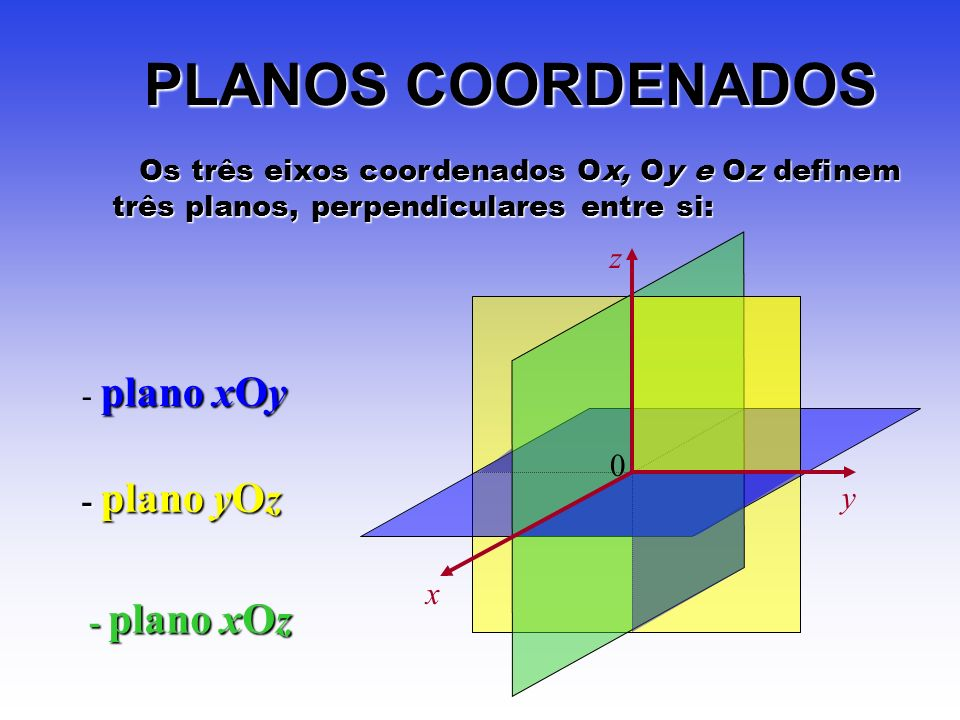
\includegraphics[height=8cm]{images/google-images_planos-coordenados}
			\end{figure}
			%------------------------------
			\tabularnewline
			\midrule
			%------------------------------
			\textbf{Quádricas}
			%------------------------------
			\tabularnewline
			\midrule
			%------------------------------
			\begin{tabular}[c]{@{}c@{}} 

				{\large Quádrica Degenerada (plano)} \\

				{\large $ax + by + cz = 0$} \\
				
			\end{tabular}

			\begin{figure}[H]
                \centering			    
            	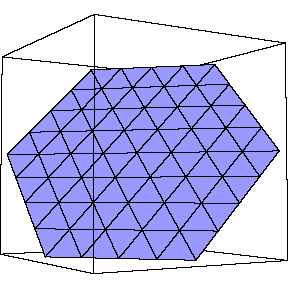
\includegraphics[height=6cm]{images/ufmg_figura-1-3}
			\end{figure}
			%------------------------------
			\tabularnewline
			\midrule
			%------------------------------
			\begin{tabular}[c]{@{}c@{}} 

				{\large Esfera (caso particular do elipsóide)} \\

				{\large $ax^{2} + by^{2} + cz^{2} = k$} \\
				
			\end{tabular}

			\begin{figure}[H]
			    \centering
				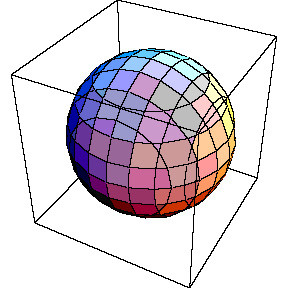
\includegraphics[height=6cm]{images/ufmg_figura-1-1}
			\end{figure}
			%------------------------------
			\tabularnewline
			\midrule
			%------------------------------
			\begin{tabular}[c]{@{}c@{}} 

				{\large Elipsóide} \\

				{\large $ax^{2} + by^{2} + cz^{2} = k$} , ($a \neq b$ ou $b \neq c$ ou $a \neq c$)\\

            \end{tabular}

			\begin{figure}[H]
			    \centering
				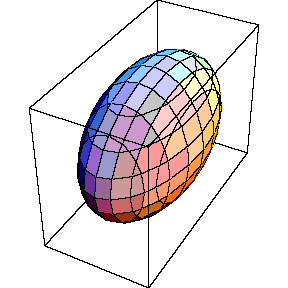
\includegraphics[height=6cm]{images/ufmg_figura-1-2}
			\end{figure}
			%------------------------------
			\tabularnewline
			\midrule
			%------------------------------
			\begin{tabular}[c]{@{}c@{}} 

				{\large Hiperbolóide} \\

				{\large $ax^{2} + by^{2} - cz^{2} = k$} \\

            \end{tabular}

			\begin{figure}[H]
			    \centering	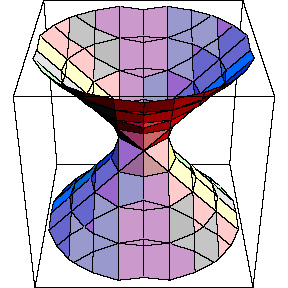
\includegraphics[height=6cm]{images/ufmg_figura-1-4}
			\end{figure}
			%------------------------------
			\tabularnewline
			\midrule
			%------------------------------
			\begin{tabular}[c]{@{}c@{}} 

				{\large Cone} \\

				{\large $ax^{2} + by^{2} - cz^{2} = 0$} \\

            \end{tabular}

			\begin{figure}[H]
			    \centering	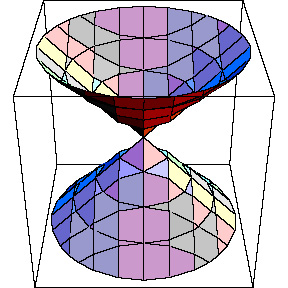
\includegraphics[height=6cm]{images/ufmg_figura-1-5}
			\end{figure}
			%------------------------------
			\tabularnewline
			\midrule
			%------------------------------
			\begin{tabular}[c]{@{}c@{}} 

				{\large Parabolóide} \\

				{\large $ax^{2} + ay^{2} = cz$}\\

            \end{tabular}

			\begin{figure}[H]
			    \centering
				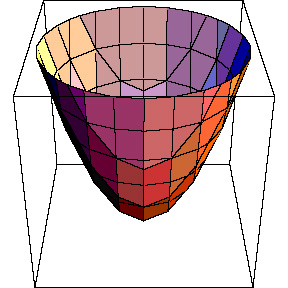
\includegraphics[height=6cm]{images/ufmg_figura-1-6}
			\end{figure}
			%------------------------------
			\tabularnewline
			\midrule
			%------------------------------
			\begin{tabular}[c]{@{}c@{}} 

				{\large Parabolóide Elíptico} \\

				{\large $ax^{2} + by^{2} = cz$}\\

            \end{tabular}

			\begin{figure}[H]
			    \centering
				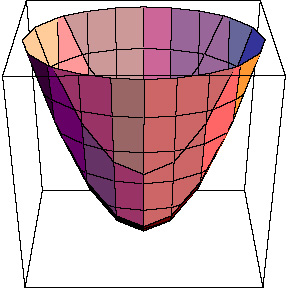
\includegraphics[height=6cm]{images/ufmg_figura-1-7}
			\end{figure}
			%------------------------------
			\tabularnewline
			\midrule
			%------------------------------
			\begin{tabular}[c]{@{}c@{}} 

				{\large Parabolóide Hiperbólico ou Sela} \\

				{\large $ax^{2} - by^{2} = cz$}\\

            \end{tabular}

			\begin{figure}[H]
			    \centering
				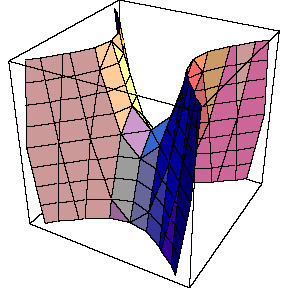
\includegraphics[height=6cm]{images/ufmg_figura-1-8}
			\end{figure}
			%------------------------------
			\tabularnewline
			\midrule
			%------------------------------
			\begin{tabular}[c]{@{}c@{}} 

				{\large Cilindro} \\

				{\large $ax^{2} - by^{2} + dx + ey = k$}\\

            \end{tabular}

			\begin{figure}[H]
			    \centering
				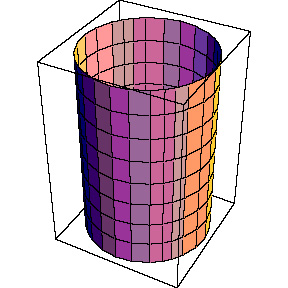
\includegraphics[height=6cm]{images/ufmg_figura-1-9}
			\end{figure}
			%------------------------------
			\tabularnewline
			\bottomrule

		\end{longtable}
		
	\subsection{Derivadas}

		\begin{longtable}{
		@{}
		C{1\textwidth} 
		@{}}

			\toprule
			%------------------------------
			\textbf{Derivadas Parciais}
			%------------------------------
			\tabularnewline
			\midrule
			%------------------------------
			{\large \begin{tabular}[c]{@{}c@{}}

				$\cfrac{\partial f}{\partial x} (x_{0}, y_{0}) = f_{x} = \lim \limits_{\Delta x \to 0} \cfrac{\Delta f}{\Delta x}$ \\

				$\cfrac{\partial f}{\partial y} (x_{0}, y_{0}) = f_{y} = \lim \limits_{\Delta y \to 0} \cfrac{\Delta f}{\Delta y}$

			\end{tabular}}
			%------------------------------
			\tabularnewline
			\midrule
			%------------------------------
			\textbf{Diferencial de uma Função}
			%------------------------------
			\tabularnewline
			\midrule
			%------------------------------
			{\large $df = f_{x} \times \Delta x + f_{y} \times \Delta y$}
			%------------------------------
			\tabularnewline
			\midrule
			%------------------------------
			\textbf{Função Composta - Regra da Cadeia}
			%------------------------------
			\tabularnewline
			\midrule
			%------------------------------
			{\large $\cfrac{dF}{dt} = \cfrac{\partial f}{\partial x} \times \cfrac{dx}{dt} + \cfrac{\partial f}{\partial y} \times \cfrac{dy}{dt}$}
			%------------------------------
			\tabularnewline
			\midrule
			%------------------------------
			\textbf{Derivadas Parciais de Segunda Ordem}
			%------------------------------
			\tabularnewline
			\midrule
			%------------------------------
			{\large \begin{tabular}[c]{@{}c@{}}

				Derivada de $fx$ em relação a $x$ \hspace{1cm} $f_{xx}$ \ ou \ $\cfrac{\partial^{2}f}{\partial x^{2}}$ \\

				Derivada de $fx$ em relação a $y$ \hspace{1cm} $f_{xy}$ \ ou \ $\cfrac{\partial^{2}f}{\partial y\partial x}$ \\

				Derivada de $fy$ em relação a $x$ \hspace{1cm} $f_{yx}$ \ ou \ $\cfrac{\partial^{2}f}{\partial x\partial y}$ \\

				Derivada de $fy$ em relação a $y$ \hspace{1cm} $f_{yy}$ \ ou \ $\cfrac{\partial^{2}f}{\partial y^{2}}$

			\end{tabular}}
			%------------------------------
            \tabularnewline
			\bottomrule

		\end{longtable}

	\subsection{Funções Financeiras/Administrativas}

		\begin{longtable}{
		@{}
		C{1\textwidth} 
		@{}}

			\toprule
			%------------------------------
			\textbf{Função de Cobb-Douglas}
			%------------------------------
			\tabularnewline
			\midrule
			%------------------------------
			{\large $P = f(L, K) = A \times K^{\alpha} \times L^{1 - \alpha}$}
			%------------------------------
			\tabularnewline
			\bottomrule

		\end{longtable}
		
	\subsection{Integrais $(\int)$}

		\begin{longtable}{
		@{}
		C{1\textwidth} 
		@{}}

			\toprule
			%------------------------------
			\textbf{Integrais Parciais}
			%------------------------------
			\tabularnewline
			\midrule
			%------------------------------
			{\large \begin{tabular}[c]{@{}c@{}}

				Integral parcial em relação a $x$ \hspace{1cm} $\int f(x, y) dx$ \\

				Integral parcial em relação a $y$ \hspace{1cm} $\int f(x, y) dy$


			\end{tabular}}
			%------------------------------
			\tabularnewline
			\midrule
			%------------------------------
			\textbf{Integrais Duplas}
			%------------------------------
			\tabularnewline
			\midrule
			%------------------------------
			{\large \begin{tabular}[c]{@{}c@{}}

				$A(x) = \int \limits^{d}_{c} f(x, y)dy$ \hspace{1cm} $V = \int \limits^{b}_{a} A(x)dx$ \\

				$B(y) = \int \limits^{b}_{a} f(x, y)dx$ \hspace{1cm} $V = \int \limits^{d}_{c} B(y)dy$

			\end{tabular}}
			%------------------------------
			\tabularnewline
			\midrule
			%------------------------------
			{\large \begin{tabular}[c]{@{}c@{}}

				$\iint_{D} f(x, y)dxdy = \int \limits^{b}_{a} \left[ \int \limits^{d}_{c} f(x, y)dx \right] dy$ \\

				$\iint_{D} f(x, y)dydx = \int \limits^{d}_{c} \left[ \int \limits^{b}_{a} f(x, y)dy \right] dx$

			\end{tabular}}
			%------------------------------
			\tabularnewline
			\bottomrule

		\end{longtable}

	\subsection{Estudo de Funções de 2 Variáveis}

		\begin{longtable}{
		@{}
		C{1\textwidth} 
		@{}}

			\toprule
			%------------------------------
			\textbf{Pontos Críticos}
			%------------------------------
			\tabularnewline
			\midrule
			%------------------------------			
			{\large $fx(x_{0}, y_{0}) = 0$ e $fy(x_{0}, y_{0}) = 0$}
			%------------------------------
			\tabularnewline
			\midrule
			%------------------------------
			\textbf{Pontos de Máximo ou Mínimo}
			%------------------------------
			\tabularnewline
			\midrule
			%------------------------------
			{\large \begin{tabular}[c]{@{}c@{}}

				$
				H(x_{0}, y_{0}) =
				\begin{vmatrix}

					f_{xx}(x_{0}, y_{0}) & f_{xy}(x_{0}, y_{0}) \\
					f_{yx}(x_{0}, y_{0}) & f_{yy}(x_{0}, y_{0})
					\end{vmatrix}
				$ \\

				$H(x_{0}, y_{0}) > 0$ e $f_{xx}(x_{0}, y_{0}) < 0$ , $(x_{0}, y_{0})$ será ponto de máximo de $f$ \\

				$H(x_{0}, y_{0}) > 0$ e $f_{xx}(x_{0}, y_{0}) > 0$, $(x_{0}, y_{0})$ será ponto de mínimo de $f$ \\

				$H(x_{0}, y_{0}) < 0$ , $(x_{0}, y_{0})$ será ponto de sela de $f$

			\end{tabular}}
			%------------------------------
			\tabularnewline
			\midrule
			%------------------------------
			{\large \begin{tabular}[c]{@{}c@{}}

				\textbf{Máximos e Mínimos Condicionados} \\

				\textbf{Método dos Multiplicadores de Lagrange}

			\end{tabular}}
			%------------------------------
			\tabularnewline
			\midrule
			%------------------------------
			{\large Não se aplica se \hspace{1cm} $\cfrac{\partial \Phi}{\partial x} (x_{0}, y_{0}) = 0$ \ e \ $\cfrac{\partial \Phi}{\partial y} (x_{0}, y_{0}) = 0$}
			%------------------------------
			\tabularnewline
			\midrule
			%------------------------------
			{\large \begin{tabular}[c]{@{}c@{}}

				$F(x, y, \lambda) = f(x, y) - \lambda \times \Phi (x, y)$ \\

				$\cfrac{\partial F}{\partial x} = 0$ \hspace{1cm} $\cfrac{\partial F}{\partial y} = 0$ \hspace{1cm} $\cfrac{\partial F}{\partial \lambda} = 0$

			\end{tabular}}
			%------------------------------
			\tabularnewline
			\midrule
			%------------------------------
			{\large \begin{tabular}[c]{@{}c@{}}

				$\cfrac{\partial f}{\partial x} (x_{0}, y_{0}) = \lambda \times \cfrac{\partial \Phi}{\partial x} (x_{0}, y_{0})$ \hspace{1cm} $\cfrac{\partial f}{\partial y} (x_{0}, y_{0}) = \lambda \times \cfrac{\partial \Phi}{\partial y} (x_{0}, y_{0})$ \\

				$\cfrac{\partial f}{\partial x} = \lambda \times \cfrac{\partial \Phi}{\partial x}$ \hspace{1cm} $\cfrac{\partial f}{\partial y} = \lambda \times \cfrac{\partial \Phi}{\partial y}$ \hspace{1cm} $\Phi (x, y) = 0$

			\end{tabular}}
			%------------------------------
			\tabularnewline
			\bottomrule

		\end{longtable}

	\part{Pré-Cálculo}

		\section{Números Irracionais e Constantes Naturais}

		\section{Produtos Notáveis}

		\section{Progressões}

		\section{Logaritmos}

		\section{Trigonometria}

	\part{Cálculo Univariado}

		\section{Função Polinomial}

	\subsection{Definição}
	
	Uma função polinomial $ f : \mathbb{R} \rightarrow \mathbb{R} $ de grau $ n $ é uma função da forma
	
	\bigskip
	
	{\Large $ y = f'(x) = a_{n} x^{n} + a_{n-1} x^{n-1} + \dots + a_{3} x^{3} + a_{2} x^{2} + a_{1} x + a_{0} $}
	
	\bigskip
	
	onde
	
	$ n $ é o grau do polinômio; \\
	$ a_{n}, a_{n-1}, \dots , a_{3}, a_{2}, a_{1}, a_{0} $ são constantes reais $ a_{n} \neq 0 $; \\
	$ x $ é a variável independente; \\
	$ y = f(x) $ é a variável dependente;
	
	\subsection{Função do 1º Grau}
	
	{\Large $ y = ax + b $}
	
	\bigskip
	
	onde $ a = m $ é o coeficiente angular e $ b $ o coeficiente linear.
	
	\bigskip
	
	{\Large $ m = \cfrac{\Delta y}{\Delta x} = \cfrac{y_2 - y_1}{x_2 - x_1}$}
	
	
	\subsection{Equação Quadrática (Fórmula de Bhaskara)}
	
	{\Large $ ax^{2} + bx + c = 0 $}
	
	\bigskip
	
	onde
	
	\bigskip
	
	{\Large $ x = \cfrac {-b \pm \sqrt {b^2 - 4ac}} {2a} $}

		\subsubsection{Discriminante da equação quadrática}
	
		{\Large $ \Delta = b^{2} - 4ac $}
		
		\bigskip
		
		Se $ \Delta > 0 $ a equação tem duas raízes reais e distintas \\
		Se $ \Delta = 0 $ a equação tem duas raízes reais e iguais (tecnicamente chamada de raiz dupla), ou popularmente "uma única raiz". \\
		Se $ \Delta < 0 $ a equação não possui qualquer raiz real.
		
		\subsubsection{Sentido da parábola}
		
		Caso $ a > 0 $ a parábola terá o aspecto de côncava para baixo (ou somente côncava). \\
		Caso $ a < 0 $ a parábola terá aspecto de côncava para cima (ou convexa).

		\section{Função Modular de um Número Real}

	\begin{Large}
	$ |x| = x$, se $x>=0 $ \\
	ou\\
	$ |x| = -x$, se $x<0 $	
	\end{Large}

	\
	
	e.g. \ $2 \cdot |3| = 2 \cdot (3) = 6$\\
	e.g. \ $|-4| + |-2| = -(-4) + [- (-2)] = 4 + 2 = 6$
	
		\section{Limites}

	\subsection{Sucessões ou Sequências \cite{morettin}}

	\subsection{Convergência de Sucessões \cite{morettin}}

	\subsection{Limite de Funções \cite{morettin}}

	\subsection{Propriedades Operatórias \cite{somatematica} \cite{ventura}}

		As propriedades operatórias permitem achar os limites de somas, diferenças, produtos, quocientes e outros mais de funções elementares.
		
		Para funções $f$ e $g$ com limites para $x \to a$, $\lim \limits_{x \to a} f(x) = L$ e $\lim \limits_{x \to a} g(x) = M$, desde que $(L, M \neq \infty )$, temos:

		\medskip

		\begin{enumerate}[label=(P\arabic*)]

			\item {\LARGE $\lim \limits_{x \to a} [f(x) \pm g(x)] = \lim \limits_{x \to a} f(x) \pm \lim \limits_{x \to a} g(x)$}

			\medskip

			\textbf{Exemplo}: $\lim \limits_{x \to 1} [x^{2} + 3x^{3}] = \lim \limits_{x \to 1} x^{2} + \lim \limits_{x \to 1} 3x^{3} = 1 + 3 = 4$ ;

			\item {\LARGE $\lim \limits_{x \to a} [f(x) \times g(x)] = \lim \limits_{x \to a} f(x) \times \lim \limits_{x \to a} g(x)$}

			\medskip

			\textbf{Exemplo}: $\lim \limits_{x \to \pi} [3x^{3} \times \cos x] = \lim \limits_{x \to \pi} 3x^{3} \times \lim \limits_{x \to \pi} \cos x = 3\pi ^{3} \times cos \pi = 3 \pi ^{3} \times (-1) = - 3 \pi ^{3}$ ;

			\item {\LARGE $\lim \limits_{x \to a} \cfrac{f(x)}{g(x)} = \cfrac{\lim \limits_{x \to a} f(x)}{\lim \limits_{x \to a} g(x)}$, desde que $\lim \limits_{x \to a} g(x) \neq 0$}

			\medskip

			\textbf{Exemplo}: $\lim \limits_{x \to 0} \cfrac{\cos x}{x^{2} + 1} = \cfrac{\lim \limits_{x \to 0} \cos x}{\lim \limits_{x \to 0} x^{2} + 1} = \cfrac{\cos 0}{0^{2} + 1} = \cfrac{1}{1} = 1$ ;

			\item {\LARGE $\lim \limits_{x \to a} f(x)^{n} = \left( \lim \limits_{x \to a} f(x) \right) ^{n}$, desde que $n \in \mathbb{N}^{*}$}

			\medskip

			\textbf{Exemplo}: $\lim \limits_{x \to 1} (x^{2} + 3)^{2} = \left[ \lim \limits_{x \to 1} (x^{2} + 3)^{2} \right] = (1 + 3)^{2} = 16$ ;

			\item {\LARGE $\lim \limits_{x \to a} \sqrt[n]{f(x)} = \sqrt[n]{\lim \limits_{x \to a} f(x)}$, desde que $n \in \mathbb{N}^{*}$ e $f(x) > 0$ (se $f(x) \leq 0$ $n$ é ímpar)}

			\medskip

			\textbf{Exemplo}: $\lim \limits_{x \to 2} \sqrt{x^{3} + x^{2} - 1} = \sqrt{\lim \limits_{x \to 2} x^{3} + x^{2} - 1} = \sqrt{2^{3} + 2^{2} - 1} = \sqrt{11}$ ;

			\item {\LARGE $\lim \limits_{x \to a} (\ln f(x)) = \ln \left[ \lim \limits_{x \to a} f(x) \right]$, desde que $\lim \limits_{x \to a} f(x) > 0$}

			\medskip

			\textbf{Exemplo}: $\lim \limits_{x \to e} (\ln x^{2}) = \ln \left[ \lim \limits_{x \to e} x^{2} \right] = \ln e^{2} = 2 \ln e = 2 \times 1 = 2$ ;

			\item {\LARGE $\lim \limits_{x \to a} \sin (f(x)) = \sin \left( \lim \limits_{x \to a} f(x) \right)$}

			\medskip

			\textbf{Exemplo}: $\lim \limits_{x \to 1} \sin (x^{2} + 3x) = \sin \left[ \lim \limits_{x \to 1} (x^{2} +3x) \right] = \sin 4$ ;

			\item {\LARGE $\lim \limits_{x \to a} e^{f(x)} = e^{\lim \limits_{x \to a} f(x)}$}

			\medskip

			\textbf{Exemplo}: $\lim \limits_{x \to 1} e^{x^{2} + 3x} = e^{\lim \limits_{x \to 1} x^{2} +3x} = e^{4}$ .

		\end{enumerate}

	\subsection{Formas Indeterminadas \cite{morettin}}

	\subsection{Limites Infinitos \cite{morettin}}

	\subsection{Limites nos Extremos do Domínio \cite{morettin}}

	\subsection{Continuidade de uma Função \cite{morettin}}

	\subsection{Assíntotas Verticais e Horizontais \cite{morettin}}

	\subsection{Limite Exponencial Fundamental \cite{morettin}}
	
		\section{Derivadas}
	
		\section{Aplicações de Derivadas}
	
		\section{Integrais ( $\int$ )}

	\subsection{Integral Indefinida \cite{morettin}}

		\subsubsection{Definição \cite{morettin}}
	
			Chamamos de integral indefinida de $ g(x) $ e indicamos pelo símbolo $ \int g(x) \ dx $ a uma primitiva qualquer de $ g(x) $ adicionada a uma constante arbitrária $ c $. Assim:
			
			\bigskip
	
			{\LARGE $\int g(x)dx = f(x) + c $} \ ,
			
			\bigskip
	
			em que $ f(x) $ \footnote{Lucchesi \cite{lucchesi} utiliza a notação $ F(x) $ para representar funções primitivas.} é uma primitiva de $ g(x) $ , ou seja, $ f'(x) = g(x) $ \cite{morettin}
	
		\subsubsection{Funções Elementares \cite{morettin}}
	
			Podemos obter as integrais indefinidas das principais funções, que decorrem imediatamente das respectivas regras de derivação:
	
			\begin{enumerate}[label=(\alph*)]

				\item Se $ n $ é inteiro e diferente de $ -1 $ , então {\LARGE $\int x^{n} dx = \cfrac {x^{n + 1}} {n+1} + c $} , pois a derivada de $ \cfrac {x^{n + 1}} {n+1} $ é $ x^{n} $ .

				\item $\int \cfrac {1} {x} \ dx = \ln x + c $ , para $ x > 0 $ , pois a derivada de $ \ln x $ é $ \cfrac {1} {x} $ .
			
				observemos que se $ x < 0 $ , $ \int \cfrac {1} {x} \ dx = \ln (-x) + c $ . Assim, de modo geral, podemos escrever:

				\bigskip

				{\LARGE $\int \frac {1} {x} \ dx = \ln |x| + c$} .

				\item Para qualquer real $\alpha \neq -1$ , {\Large $\int x^{a} \ dx = \cfrac {x^{\alpha + 1}} {\alpha + 1} + c$} . \ $(x > 0)$
			
				\item {\LARGE $\int \cos xdx = \sin x + c$} , pois a derivada de $ \sin x $ é $ \cos x $ .

				\item {\LARGE $\int \sin xdx = - \cos x + c$} , pois a derivada de $- \cos x$ é $\sin x$ .

				\item {\LARGE $\int e^{x} \ dx = e^{x} + c$} , pois a derivada de $e^{x} $ é $e^{x}$ .

				\item {\LARGE $\int \cfrac {1}{1+x^{2}} \ dx = \arctan x + c$} , pois a derivada de $\arctan x$ é $\cfrac {1}{1+x^{2}}$ .

				\item {\LARGE $\int \cfrac {1}{\sqrt{1 - x^{2}}} \ dx = \arcsin x + c$} , pois a derivada de $\arcsin x$ é $\cfrac {1}{\sqrt{1 - x^{2}}} $ , para $ -1 < x < 1$ .
				
			\end{enumerate}
	
		\subsubsection{Propriedades Operatórias \cite{morettin}}
	
			\begin{enumerate}[label=(P\arabic*)]
			
				\item {\LARGE $\int [ f_{1} (x) + f_{2} (x) ] \ dx = \int f_{1} (x) \ dx + \int f_{2} (x) \ dx$} ;
			
				\item {\LARGE $\int [ f_{1} (x) - f_{2} (x) ] \ dx = \int f_{1} (x) \ dx - \int f_{2} (x) \ dx$} ;
			
				\item {\LARGE $\int c \cdot f(x) \ dx = c \cdot \int f(x) \ dx$} .
		
			\end{enumerate}
	
	\subsection{Integral Definida \cite{morettin}}

		\subsubsection{Definição \cite{morettin}}
	
			Seja $ f(x) $ uma função e $ g(x) $ uma de suas primitivas. Portanto, $ \int f(x) \ dx = g(x) + c $ .

			Definimos a integral definida de $ f(x) $ entre os limites $ a $ e $ b $ como a diferença $ g(b) - g(a) $ , e indicamos simbolicamente
			
			\bigskip

			{\LARGE $ \int_{a}^{b} f(x) \ dx = g(b) - g(a) = \lim \limits_{x \to b-} [g(x)] - \lim \limits_{x \to a+} [g(x)] $} .

			\bigskip

			A diferença $ g(b) - g(a) $ também costuma ser indicada pelo símbolo $ [g(x)]_{a}^{b} $.
	
		\subsubsection{Teorema Fundamental do Cálculo \cite{morettin}}
	
			O significado geométrico da integral definida é dado a seguir.

			Seja $ f(x) $ uma função \textbf{contínua e não negativa} definida num intervalo $ [a, b] $ . A integral definida $ \int_{a}^{b} f(x) \ dx $ representa a área da região compreendida entre o gráfico de $ f(x) $ , o eixo $ x $ e as verticais que passam por $ a $ e $ b $ .

			\bigskip

			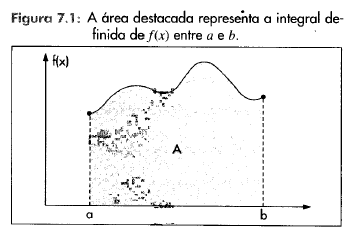
\includegraphics[height=6cm]{images/morettin_figura-7-1}

			Assim, indicado por \textbf{$ A $} a área destacada da Figura 7.1, teremos:
			
			\bigskip

			{\LARGE $A = \int_{a}^{b} f(x) \ dx$}
	
			\bigskip
			
			(...) Caso $ f(x) $ seja negativa no intervalo $ [a, b] $ , a área $ A $ da região delimitada pelo gráfico de $ f(x) $ , eixo $ x $ , e pelas verticais que passam por $ a $ e por $ b $ é dada por:

			\bigskip

			{\LARGE $A = - \int_{a}^{b} f(x) \ dx$} .

		\subsubsection{Propriedades Operatórias \cite{lucchesi}}
		
			\begin{enumerate}[label=(P\arabic*)]
			
				\item {\Large $\int_{a}^{a} f(x) \ dx = F(a) - F(a) = 0$}
				
				\item {\Large $\int_{a}^{b} f(x) \ dx = - \int_{b}^{a} f(x) \ dx$}
			
				\item {\Large $\int_{a}^{b} f(x) \ dx = \int_{a}^{c} f(x) \ dx + \int_{c}^{b} f(x) \ dx $} , sendo $ a < c < b$ .
		
			\end{enumerate}
	
	\subsection{Integral Imprópria \cite{lucchesi}}
	
		\subsubsection{Definição \cite{lucchesi}}
	
			Quando as hipóteses do teorema fundamental do cálculo falharem, aplicamos a integral imprópria.
		
			Caso 1: Intervalo de integração aberto (e.g. ]a, b]).
			
			Caso 2: Descontinuidade da função (e.g. $ D = \mathbb{R} - (0) $ ).
		
			Usa-se a propriedade da integral definida:
		
			\begin{enumerate}[label=(P3)]
			
				\item {\LARGE $\int_{a}^{b} f(x) \ dx = \int_{a}^{c} f(x) \ dx + \int_{c}^{b} f(x) \ dx $ , sendo $ a < c < b $} .
		
			\end{enumerate}

			\medskip		

			\textbf{Exemplo}:

				\medskip

				$\int_{-1}^{1} \frac {1}{x^2} \ dx \ \longrightarrow \ D = \mathbb{R} - (0) $
			
				\bigskip
			
				$ \int_{-1}^{1} \frac {1}{x^2} \ dx = \lim \limits_{z \to 0^{-}} \int_{-1}^{z} \frac {1}{x^2} \ dx + \lim \limits_{z \to 0^{+}} \int_{z}^{1} \frac {1}{x^2} \ dx $
	
	\part{Cálculo Multivariado}

		\section{O Espaço n-Dimensional ( $ \mathbb{R}^{n} $ )}

	\subsection{O Espaço Bidimensional \cite{morettin}}

		``Seja $\mathbb{R}$ o conjunto dos números reais. O conjunto formado por todos os pares ordenados de reais é chamado \textbf{espaço bidimensional} e é indicado por $\mathbb{R} \times \mathbb{R}$ ou simplesmente $\mathbb{R}^{2}$":

		\bigskip

		{\LARGE $\mathbb{R}^{2} = \{(a, b) \ | \ a \in \mathbb{R} \ \text{e} \ b \in \mathbb{R} \}$}
		
		\bigskip		
		
		``Geometricamente, um elemento $(a, b)$ de $\mathbb{R}^{2}$ pode ser representado no plano cartesiano por um ponto de abscissa $a$ e ordenada $b$".		
		
		\begin{figure}[H]
			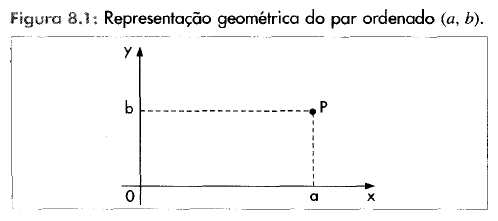
\includegraphics[height=5cm]{images/morettin_figura-8-1}
		\end{figure}
		
	\subsection{Relações em $\mathbb{R}^{2}$ \cite{morettin}}
	
		``Chama-se \textbf{relação binária}, ou simplesmente relação no $\mathbb{R}^{2}$, a todo conjunto de $\mathbb{R}^{2}$".

		\bigskip

		``\textbf{Exemplo 8.2}. Seja $A = \{(x, y) \in \mathbb{R}^{2} | y = 2x + 1 \}$. A representação geométrica do conjunto $A$ é uma reta"

		\begin{figure}[H]
			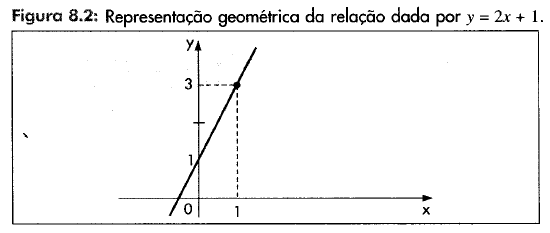
\includegraphics[height=5cm]{images/morettin_figura-8-2}
		\end{figure}

		``\textbf{Exemplo 8.3}. Considerando $C = \{(x, y) \in \mathbb{R}^{2} \ | \ x^{2} + y^{2} \leq 4\}$, a representação geométrica do conjunto $C$ é um círculo de centro na origem e raio $2$ (Figura 8.4)".

		\begin{figure}[H]
			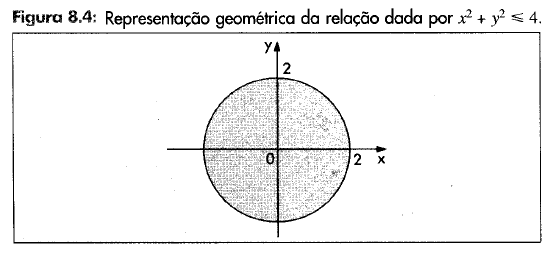
\includegraphics[height=5cm]{images/morettin_figura-8-4}
		\end{figure}

		\textbf{Observação}

		Lembremos que, se tivermos no plano cartesiano a representação gráfica de uma função $y = f(x)$, os pontos que estão ``acima" do gráfico satisfazem a relação $y > f(x)$.

		No caso de termos a representação geométrica de uma circunferência de equação $(x - a)^{2} + (y - b)^{2} = r^{2}$, de centro $C(a, b)$ e raio $r$, os pontos interiores a ela satisfazem a relação $(x - a)^{2} + (y - b)^{2} < r^{2}$, e os pontos exteriores a ela satisfazem a relação $(x - a)^{2} + (y - b)^{2} > r^{2}$.

		Uma relação do tipo $x  > k$ é representada geometricamente pelos pontos do plano à direita da reta vertical $x = k$; a relação $x < k$ é representada pelos pontos à esquerda da reta vertical $x = k$.

	\subsection{Equação do Círculo \cite{wikipedia}}

		Em um sistema cartesiano bidimensional $\mathbb{R}^{2}$, um círculo com as coordenadas de centro $(a, b)$ e raio $r$ se dá pelo conjunto de todos os pontos $(x, y)$ tal que

		\bigskip

		{\LARGE $(x - a)^{2} + (y - b)^{2} = r^{2}$} .

		\bigskip

		Esta equação, conhecida como a equação do círculo, segue o teorema de Pitágoras aplicado a qualquer ponto no círculo - como demonstrado no diagrama abaixo, o raio é a hipotenusa de um triângulo reto que tem como catetos $|x - a|$ e $|y - b|$. Se o círculo está centrado na origem $(0, 0)$, a equação se simplifica para

		\bigskip

		{\LARGE $x^{2} + y^{2} = r^{2}$} .

		\begin{figure}[H]
			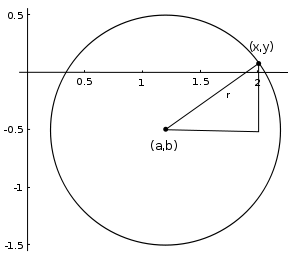
\includegraphics[height=5cm]{images/wikipedia_circle-equation}
		\end{figure}
		
	\subsection{Distância entre Dois Pontos em $\mathbb{R}^{2}$ \cite{morettin}}

		``Sejam $(x_{1}, y_{1})$ e $(x_{2}, y_{2})$ dois elementos de $\mathbb{R}^{2}$, representados geometricamente pelos pontos $P_{1}$ e $P_{2}$. A distância entre eles é o número

		\bigskip

		{\LARGE $d(P_{1}, P_{2}) = \sqrt{(x_{2} - x_{1})^{2} + (y_{2} - y_{1})^{2}}$} [Teorema de Pitágoras].

		\bigskip

		Notemos que a distância representa o comprimento do segmento $\overline{P_{1}P_{2}}$ na representação geométrica (Figura 8.7). Quando não houver possibilidade de confusão, a distância é indicada simplesmente por $d$".

		\begin{figure}[H]
			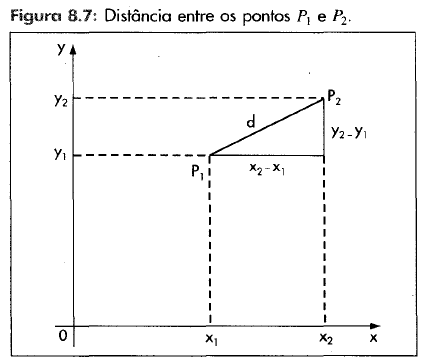
\includegraphics[height=7cm]{images/morettin_figura-8-7}
		\end{figure}

	\subsection{O Espaço Tridimensional \cite{morettin}}

		Seja $\mathbb{R}$ o conjunto dos números reais. O conjunto formado por todas as triplas ordenadas de reais é chamado \textbf{espaço tridimensional} e é indicado por $\mathbb{R} \times \mathbb{R} \times \mathbb{R}$ ou simplesmente $\mathbb{R}^{3}$. Assim:

		\bigskip

		{\LARGE $\mathbb{R}^{3} = \{(a, b, c) \ | \ a \in \mathbb{R}, \ b \in \mathbb{R}, \ c \in \mathbb{R} \}$} .
		
		\bigskip		
		
		Geometricamente, um elemento $(a, b, c)$ pode ser representado por um ponto $P$ de abscissa $a$, ordenada $b$ e cota $c$, num sistema de eixos $Ox$, $Oy$ e $Oz$ perpendiculares dois a dois. A cota $c$ é a distância do ponto $P$ em relação ao plano determinado pelos eixos $Ox$ e $Oy$, precedida pelo sinal $+$ se o ponto estiver "acima" do plano, e precedida pelo sinal $-$ se estiver "abaixo" desse plano (Figura 8.8).
		
		\begin{figure}[H]
			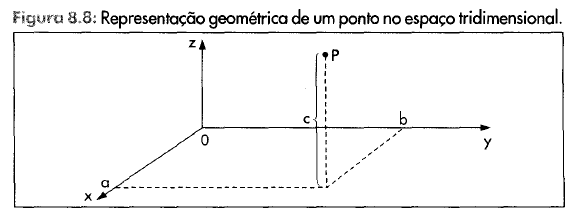
\includegraphics[height=5cm]{images/morettin_figura-8-8}
		\end{figure}

	\subsection{Relações em $\mathbb{R}^{3}$ \cite{morettin}}

		Chama-se relações no $\mathbb{R}^{3}$ a todo conjunto do $\mathbb{R}^{3}$.

		\bigskip

		\textbf{Exemplo 8.7}. Seja $A = \{(x, y, z) \ | \ x = 0 \}$, a representação geométrica de $A$ é o plano determinando pelos eixos $Oy$ e $Oz$ (Figura 8.9)

		\begin{figure}[H]
			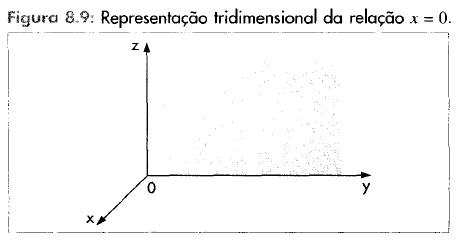
\includegraphics[height=5cm]{images/morettin_figura-8-9}
		\end{figure}

		\textbf{Exemplo 8.8}. Seja $B = \{(x, y, z) \ | \ z = 2 \}$, a representação geométrica desse conjunto é o plano paralelo determinando por $Ox$ e $Oy$ e distante duas unidades do mesmo (Figura 8.10)

		\begin{figure}[H]
			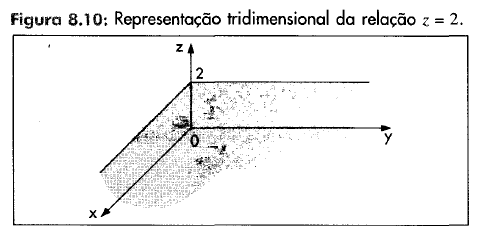
\includegraphics[height=5cm]{images/morettin_figura-8-10}
		\end{figure}

	\subsection{Equação do Plano em $\mathbb{R}^{3}$ \cite{morettin}}

		Pode se provar que toda relação do $\mathbb{R}^{3}$ que satisfaz uma equação do tipo $ax + bx + cz + d = 0$ (com $a, b, c, d$ reais e $a, b, c$ não nulos simultaneamente) tem por representação geométrica um plano no espaço tridimensional. O gráfico \textbf{por onde passa} tal plano pode ser obtido por meio de três pontos não alinhados.

		\begin{figure}[H]
			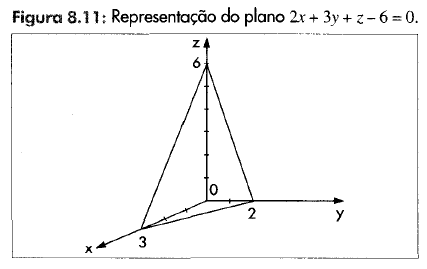
\includegraphics[height=6cm]{images/morettin_figura-8-11}
		\end{figure}

	\subsection{Distância entre Dois Pontos em $\mathbb{R}^{3}$ \cite{morettin}}

		Sejam $(x_{1}, y_{1}, z_{1})$ e $(x_{2}, y_{2}, z_{2})$ dois elementos de $\mathbb{R}^{3}$ representados pelos pontos $P_{1}$ e $P_{2}$. Chama-se a distância entre eles o número

		\bigskip

		{\LARGE $d(P_{1}, P_{2}) = \sqrt{(x_{2} - x_{1})^{2} + (y_{2} - y_{1})^{2} + (z_{2} - z_{1})^{2}}$}
		
		[Teorema de Pitágoras].

		\bigskip


		Dessa forma, a distância é o comprimento do segmento $\overline{P_{1}P_{2}}$ da Figura 8.12.

		\begin{figure}[H]
			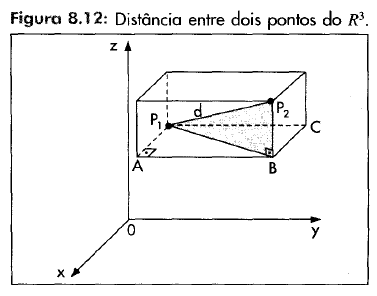
\includegraphics[height=7cm]{images/morettin_figura-8-12}
		\end{figure}

		\textbf{Dedução}

		Um dos catetos (altura) do triângulo $\overline{P_{1}BP_{2}}$ pode ser representado por $z_{2} - z_{1}$, já o outro cateto é a hipotenusa do triângulo $\overline{AP_{1}B}$ que é igual a $\sqrt{(x_{2} - x_{1})^{2} + (y_{2} - y_{1})^{2}}$. Logo temos que $d^{2} = (\sqrt{(x_{2} - x_{1})^{2} + (y_{2} - y_{1})^{2}})^{2} + (z_{2} - z_{1})^{2}$ o que simplificando fica $d(P_{1}, P_{2}) = \sqrt{(x_{2} - x_{1})^{2} + (y_{2} - y_{1})^{2} + (z_{2} - z_{1})^{2}}$.
		
	\subsection{O Conjunto $\mathbb{R}^{n}$ \cite{morettin}}

		Seja $\mathbb{R}$ o conjunto dos números reais. O conjunto formado pelas ênuplas ordenadas (sequências de $n$ elementos) de reais é chamado de espaço $n$-dimensional e é indicado por $\mathbb{R}^{n}$.

		Em particular, o conjunto $\mathbb{R}^{1}$ é o próprio conjunto dos números reais (representados geometricamente num único eixo). Os elementos de $\mathbb{R}^{n}$, pana $n > 3$, não admitem representação geométrica.

		Dado dois elementos do $\mathbb{R}^{n}$, $P_{1}(x_{1}, x_{2}, \dots , x_{n})$ e $P_{2}(y_{1}, y_{2}, \dots , y_{n})$ a distância entre eles é o número

		\bigskip

		{\LARGE $d(P_{1}, P_{2}) = \sqrt{(y_{1} - x_{1})^{2} + (y_{2} - x_{2})^{2} + \dots + (y_{n} - x_{n})^{2}}$}
		
		[Teorema de Pitágoras].
		
	\subsection{Bola Aberta \cite{morettin}}

		Seja $C$ um elemento do $R^{n}$ e $r$ um número real positivo. Chama-se bola aberta de centro $C$ e raio $r$ ao conjunto dos pontos do $R^{n}$ cuja distância até $C$ é menor que $r$. Isto é, a bola aberta é o conjunto

		\bigskip

		{\LARGE $B(C, r) = \{P \in R^{n} \mid d(P, C) < r\}$} .

		\bigskip

		\textbf{Exemplo 8.11}. A bola aberta do $\mathbb{R}^{2}$ de centro $C(4, 4)$ e raio $1$ é o interior do círculo representado na Figura 8.13.
		
		\begin{figure}[H]
			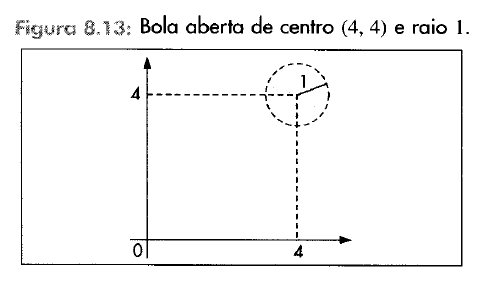
\includegraphics[height=6cm]{images/morettin_figura-8-13}
		\end{figure}

				\bigskip

		\textbf{Exemplo 8.12}. A bola aberta do $\mathbb{R}^{3}$ de centro $C(2, 3, 4)$ e raio $1$ é a região interior da esfera representada na Figura 8.14.
		
		\begin{figure}[H]
			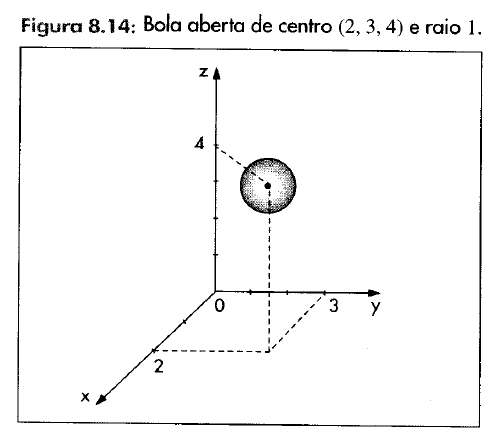
\includegraphics[height=7cm]{images/morettin_figura-8-14}
		\end{figure}
		
	\subsection{Ponto Interior \cite{morettin}}

		Seja $A$ um subconjunto do $R^{n}$; um elemento $P$ do $R^{n}$ é chamado ponto interior de $A$ se existir uma bola aberta com centro em $P$ contida em $A$. Isto é, $P$ é um ponto interior de $A$ se exisitir um real $r > 0$, tal que $B(P, r) \subset A$.

		\bigskip

		\textbf{Exemplo 8.13}. Seja $A = \{(x, y) \in \mathbb{R}^2 \mid y \geq 2\}$. O ponto $P(4, 4)$ é interior a $A$ e o ponto $P(3, 2)$ não é interior a $A$ (Figura 8.15).

		\begin{figure}[H]
			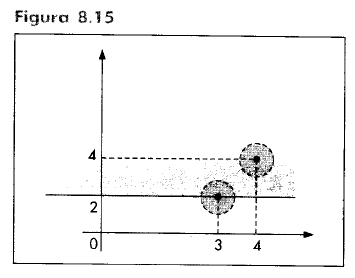
\includegraphics[height=6cm]{images/morettin_figura-8-15}
		\end{figure}
		
	\subsection{Conjunto Aberto \cite{morettin}}

		Seja $A$ um subconjunto do $\mathbb{R}^{n}$. $A$ é chamado de conjunto aberto se todos os seus pontos são interiores.

		\textbf{Exemplo 8.14}. O conjunto $A = \{(x, y) \in \mathbb{R}^2 \mid x > 2\}$ é aberto, pois todos os seus pontos são interiores (Figura 8.16).

		\begin{figure}[H]
			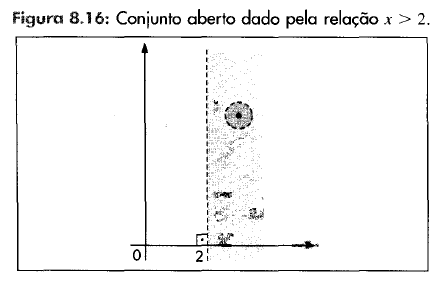
\includegraphics[height=6.5cm]{images/morettin_figura-8-16}
		\end{figure}

	\subsection{Pontos de Fronteira de um Conjunto \cite{morettin}}

		Seja $A$ um subconjunto do $\mathbb{R}^{n}$. Um ponto de $A$ que não é interior chama-se ponto de fronteira de $A$.

		\textbf{Exemplo 8.16}. Seja $A = \{(x, y) \in \mathbb{R}^2 \mid y \geq 2\}$. Os pontos da reta $y = 2$ são pontos de fronteira de $A$ (Figura 8.18).

		\begin{figure}[H]
			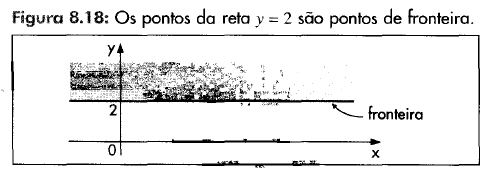
\includegraphics[height=3.5cm]{images/morettin_figura-8-18}
		\end{figure}
		
	\subsection{Planos Coordenados \cite{google}}

		Os três eixos coordenados $Ox$, $Oy$ e $Oz$ definem três planos perpendiculares entre si. Em $xOy$ temos z como constante (em que $O$ é o ponto $(0, 0, z_{0})$); em $yOz$ temos x como constante (em que $O$ é o ponto $(x_{0}, 0, 0)$); e em $xOz$ temos y como constante (em que $O$ é o ponto $(0, y_{0}, 0)$).

		\begin{figure}[H]
			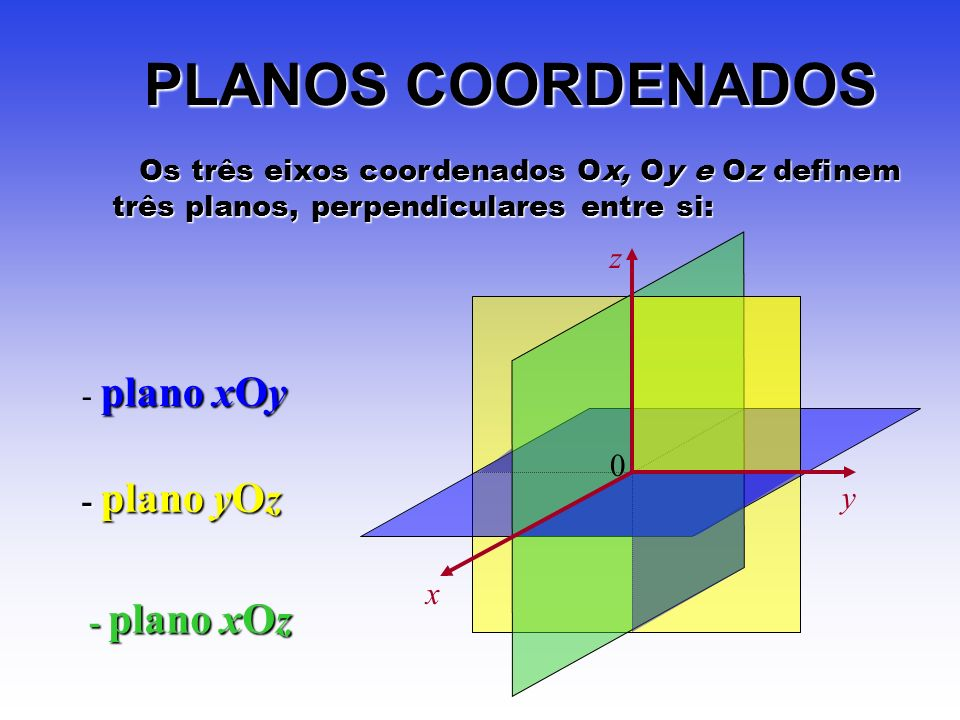
\includegraphics[height=8cm]{images/google-images_planos-coordenados}
		\end{figure}
		
		Uma das formas de criar um gráfico de um função em $\mathbb{R}^{3}$ é desenhar o cruzamento dos gráficos das funções em $xOz$ e $yOz$. Exemplo:
		
		\begin{figure}[H]
			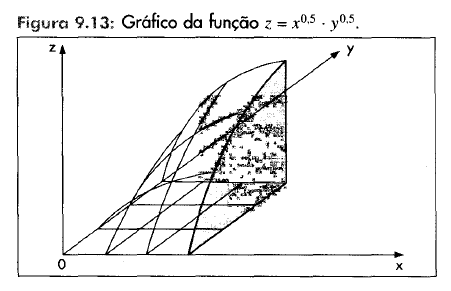
\includegraphics[height=6cm]{images/morettin_figura-9-13}
		\end{figure}

		\section{Funções de Duas Variáveis}

	\subsection{Definição \cite{morettin}}

		Seja $D$ um subconjunto do $\mathbb{R}^{2}$. Chama-se função de $D$ em $\mathbb{R}$ toda relação que associa a cada par ordenado $(x, y)$ pertencente a $D$ um único número real indicado por $f(x, y)$. O conjunto $D$ é chamado domínio da função e $f(x, y)$ é chamado de imagem de $(x, y)$ ou valor de $f$ em $(x, y)$.

	\subsection{A Função de Cobb-Douglas \cite{morettin}}

		A função de Cobb-Douglas relaciona a quantidade produzida de algum bem em certo intervalo de tempo com os insumos variáveis necessários a essa produção (trabalho, terra, capital e outros). Um modelo de função de produção muito utilizado foi introduzido pelo economista Paul Douglas e pelo matemático Charles Cobb, ambos norte-americanos, em seus estudos sobre a repartição da renda entre o capital e o trabalho no início do século XX. A expressão da referida função é

		\bigskip

		{\LARGE $P = f(L, K) = A \times K^{\alpha} \times L^{1 - \alpha}$} ,

		\bigskip

		em que

		\textbf{$P$} é a quantidade produzida, \\
		\textbf{$K$} é o capital empregado, \\
		\textbf{$L$} é a quantidade de trabalho envolvido.

		A constante \textbf{$A$} depende da tecnologia utilizada e \textbf{$\alpha$}  é um parâmetro que varia de $0$ a $1$.

	\subsection{Gráficos de Funções de Duas Variáveis \cite{morettin}}

		Vimos, no estudo de funções de uma variável, que seu gráfico era o conjunto

		\bigskip

		{\LARGE $\{(x, y) \in \mathbb{R}^{2} \mid y = f(x) \ \text{e} \ x \in D\}$} .

		\bigskip

		Consequentemente, a representação gráfica era feita no plano cartesiano (Figura 9.2).

		\begin{figure}[H]
			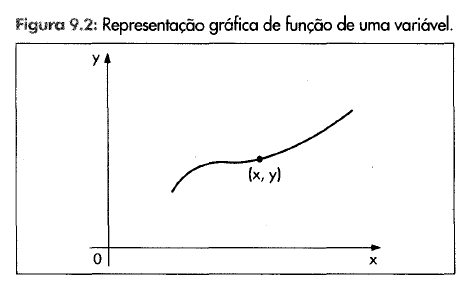
\includegraphics[height=6.5cm]{images/morettin_figura-9-2}
		\end{figure}

		De modo totalmente análogo, definimos o gráfico de uma função de duas variáveis. Seja $f(x, y)$ uma função de duas variáveis $x$ e $y$. O gráfico da função é o conjunto

		\bigskip

		{\LARGE $\{(x, y, z) \in \mathbb{R}^{3} \mid z = f(x, y) \ \text{e} \ (x, y) \in D\}$} .

		\bigskip

		Portanto o gráfico de $f(x, y)$ será representado no espaço tridimensional, de tal forma que a cada par $(x, y)$ do domínio corresponda uma cota $z = f(x, y)$, como mostra a Figura 9.3.

		\begin{figure}[H]
			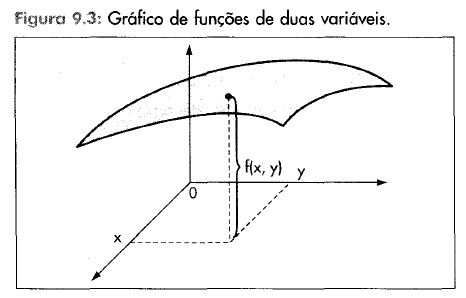
\includegraphics[height=6.5cm]{images/morettin_figura-9-3}
		\end{figure}
		
			\subsection{Curvas de Nível \cite{morettin}}

		Devido à dificuldade de desenharmos o gráfico de uma função de duas variáveis, costumamos utilizar a seguinte forma alternativa de representação: obtemos o conjunto dos pontos do domínio que têm a mesma cota $c$; tais pontos, em geral, formam uma curva que recebe o nome de curva de nível $c$ da função (Figura 9.14)

		\begin{figure}[H]
			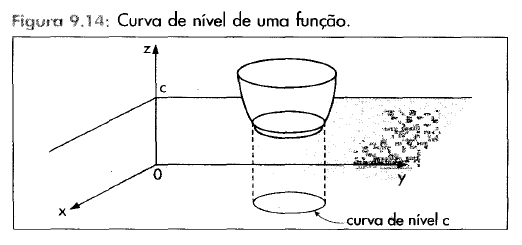
\includegraphics[height=5.5cm]{images/morettin_figura-9-14}
		\end{figure}

		Assim sendo, atribuindo valores a $c$, obtemos várias curvas de nível, que permitem tirar importantes informações sobre a função.

		O método das curvas de nível, além de ser muito utilizado em Economia, é também utilizado em outras áreas, como Engenharia (topografia de terrenos), Geografia e outras.

		\bigskip

		\textbf{Exemplo 9.9}. Seja a função $f(x, y) = x^{2} + y^{2}$. As curvas de nível $c = 1$, $c = 2$ e $c = 4$ são:

		\bigskip

		$c = 1 \Rightarrow x^{2} + y^{2} = 1$ (circunferência de centro $(0, 0)$ e raio $1$), \\
		$c = 2 \Rightarrow x^{2} + y^{2} = 2$ (circunferência de centro $(0, 0)$ e raio $\sqrt{2}$), \\
		$c = 3 \Rightarrow x^{2} + y^{2} = 4$ (circunferência de centro $(0, 0)$ e raio $2$).

		\bigskip

		Essas curvas de nível aparecem na Figura 9.15.

		\begin{figure}[H]
			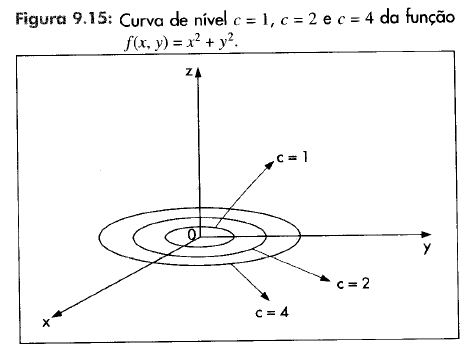
\includegraphics[height=7cm]{images/morettin_figura-9-15}
		\end{figure}

		Frequentemente, a representação das curvas de nível é feita desenhando-se apenas os eixos $0x$ e $0y$, como na Figura 9.16.


		\begin{figure}[H]
			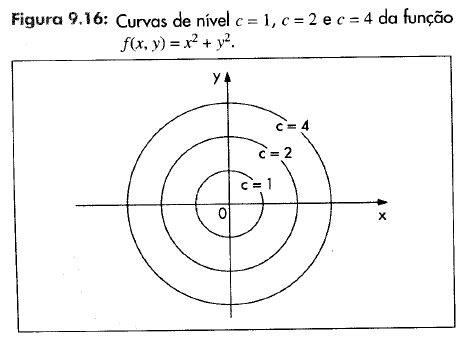
\includegraphics[height=7cm]{images/morettin_figura-9-16}
		\end{figure}
		
		\subsubsection{Curvas de Isoproduto ou Isoquantas de Produção \cite{morettin}}

			Consideremos a função de produção $P = L^{0,5} \times K^{0,5}$, em que $L$ representa o trabalho envolvido e $K$, o capital.

			As cuvas de nível $c = 1$ e $c = 2$ são:

			\medskip

			$c = 1 \Rightarrow L^{0,5} \times K^{0,5} = 1 \Rightarrow L = \cfrac{1}{K}$, \\
			$c = 2 \Rightarrow L^{0,5} \times K^{0,5} = 2 \Rightarrow L = \cfrac{4}{K}$ .

			\medskip

			A representação dessas curvas de nível comparece na Figura 9.17. Cada curva de nível fornece os pares $(K, L)$ para os quais a produção é constante, sendo a primeira com produção igual a $1$ e a segunda igual a $2$. Em Economia, essas curvas de nível são denominadas \textbf{curvas de isoproduto} ou \textbf{isoquantas de produção}.

			\begin{figure}[H]
				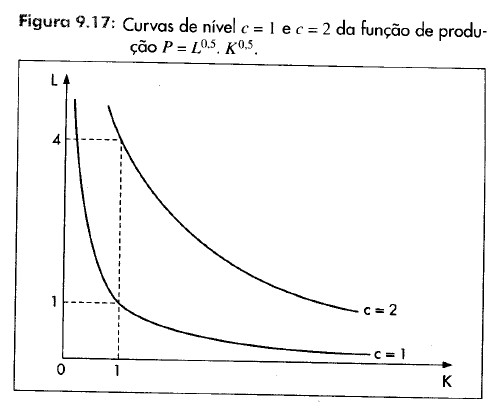
\includegraphics[height=7.5cm]{images/morettin_figura-9-17}
			\end{figure}
			
	\subsection{Limite e Continuidade \cite{morettin}}

		As noções de limite e continuidade para funções de duas variáveis são análogas às que foram vistas para funções de uma variável.

		Intuitivamente falando, o limite de $f(x, y)$ quando $(x, y)$ tende ao ponto $(x_{0}, y_{0})$ é o número $L$ (se existir) do qual se aproxima $f(x, y)$ quando $(x, y)$ se aproxima de $(x_{0}, y_{0})$, por qualquer caminho, sem no entanto ficar igual a $(x_{0}, y_{0})$.

		Indicamos essa ideia da seguinte forma:

		\bigskip

		{\LARGE $\lim \limits_{(x, y) \to (x_{0}, y_{0})} f(x, y) = L$} .

		\bigskip

		Caso $L$ seja igual a $f(x_{0}, y_{0})$, dizemos que $f$ é contínua em $(x_{0}, y_{0})$; caso contrário, $f$ é dita descontínua em $(x_{0}, y_{0})$.
		
		\subsubsection{Teorema 1 \cite{morettin}}

			São contínuas em todos os pontos de seu domínio as funções:

			\begin{enumerate}[label=(\alph*)]

				\item Polinomiais nas variáveis $x$ e $y$ ;
				\item Racionais nas variáveis $x$ e $y$ .

			\end{enumerate}

			Assim, de acordo com o Teorema 1, são contínuas por exemplo, as funções:

			\bigskip

			$f(x, y) = x^{2} + y^{2} - xy, \forall x, y$ (polinomial), \\
			$f(x, y) = x^{3}y^{2} - xy + y^{3} +6, \forall x, y$ (polinomial), \\
			$f(x, y) = \cfrac{x^{2} + y^{2}}{xy - 1}, \forall x, y \ \text{tais que} \ xy \neq 1$ (racional).
			
		\subsubsection{Teorema 2 \cite{morettin}}

			Se $f(x, y)$ e $g(x, y)$ são contínuas em $(x_{0}, y_{0})$, então serão também contínuas em $(x_{0}, y_{0})$ as funções:

			\begin{enumerate}[label=(\alph*)]

				\item $f(x, y) + g(x, y)$
				\item $f(x, y) - g(x, y)$
				\item $k \times f(x, y) \ \ (k \in \mathbb{R})$
				\item $f(x, y) \times g(x, y)$
				\item $\cfrac{f(x, y)}{g(x, y)} \ \ (g(x_{0}, y_{0}) \neq 0)$
				\item $a^{f(x, y)} \ \ (a > 0)$
				\item $\log f(x, y) \ \ (f(x_{0}, y_{0}) > 0)$
				\item $\cos f(x, y)$
				\item $\sin f(x, y)$

			\end{enumerate}

			De acordo com os teoremas vistos, são contínuas em todos os pontos de seu domínio, por exemplo, as funções:

			$f(x, y) = x^{2} + y^{2} - 2xy^{3}$ ,\\
			$f(x, y) = \cfrac{x + y}{x - y}$ ,\\
			$f(x, y) = 2^{x - y^{2}}$ ,\\
			$f(x, y) = \ln (x + y)$ ,\\
			$f(x, y) = \sin (x^{2} + y)$ ,\\
			$f(x, y) = x^{2} + e^{x}$ .

		\section{Derivadas para Funções de Duas Variáveis}

	\subsection{Derivadas Parciais \cite{morettin}}

		Consideremos um ponto $(x_{0}, y_{0})$; se mantivermos $y$ constante no valor $y_{0}$ e variarmos $x$ do valor $x_{0}$ para  o valor $x_{0} + \Delta x$, a função $f(x_{0}, y_{0})$ dependerá apenas da variável $x$.

		\medskip

		Seja

		\bigskip

		$\Delta f = f(x_{0} + \Delta x, y_{0}) - f(x_{0}, y_{0})$.

		\bigskip

		À razão
		
		\bigskip
		
		$\cfrac{\Delta f}{\Delta x} = \cfrac{f(x_{0} + \Delta x, y_{0}) - f(x_{0}, y_{0})}{\Delta x}$.

		\bigskip

		chamamos de taxa média de variação de $f$ em relação a $x$.

		\medskip

		Observemos que:
		
		\begin{enumerate}[label=(\alph*)]

			\item $\cfrac{\Delta f}{\Delta x}$ depende do ponto de partida $(x_{0}, y_{0})$;
			\item $\cfrac{\Delta f}{\Delta x}$ depende da variação $\Delta x$.

		\end{enumerate}

		Ao limite (se existir e for um número real) de $\cfrac{\Delta f}{\Delta x}$ , quando $\Delta x$ tende a $0$, denominamos derivada parcial de $f$ no ponto $(x_{0}, y_{0})$, em relação a $x$. Indicamos a tal derivada parcial por um dos símbolos:

		\bigskip

		$\cfrac{\partial f}{\partial x} (x_{0}, y_{0})$ \ \ \ ou \ \ \ $f_{x}(x_{0}, y_{0})$ .
		
		\bigskip

		Assim,

		\bigskip

		{\LARGE $\cfrac{\partial f}{\partial x} (x_{0}, y_{0}) = f_{x}(x_{0}, y_{0}) = \lim \limits_{\Delta x \to 0} \cfrac{\Delta f}{\Delta x}$} .

		\bigskip

		O símbolo $\cfrac{\partial f}{\partial x}$ (lê-se del $f$, del $x$) foi introduzido por Lagrange (Joseph Louis Lagrange, 1736-1813, matemático nascido na Itália, mas que viveu a maior parte da vida na França).

		Analogamente, se mantivermos $x$ constante no valor $x_{0}$ e variarmos $y$ do valor $y_{0}$ para o valor $y_{0} + \Delta y$, $f$ dependerá apenas da variável $y$.

		\medskip

		Seja

		\bigskip

		$\Delta f = f(x_{0}, y_{0} + \Delta y) - f(x_{0}, y_{0})$.

		\bigskip

		À razão
		
		\bigskip
		
		$\cfrac{\Delta f}{\Delta y} = \cfrac{f(x_{0}, y_{0} + \Delta y) - f(x_{0}, y_{0})}{\Delta y}$.

		\bigskip

		chamamos de taxa média de variação de $f$ em relação a $y$.

		Ao limite (se existir e for um número real) de $\cfrac{\Delta f}{\Delta y}$ quando $\Delta y$ tente a $0$, denominamos derivada parcial de $f$ no ponto $(x_{0}, y_{0})$, em relação a $y$. Indicamos tal derivada parcial por um dos símbolos:

		\bigskip

		$\cfrac{\partial f}{\partial y} (x_{0}, y_{0})$ \ \ \ ou \ \ \ $f_{y}(x_{0}, y_{0})$ .

		\bigskip

		O símbolo $\cfrac{\partial f}{\partial y}$ (lê-se del $f$, del $y$).

		\bigskip

		Assim,

		\bigskip

		{\LARGE $\cfrac{\partial f}{\partial y} (x_{0}, y_{0}) = f_{y}(x_{0}, y_{0}) = \lim \limits_{\Delta y \to 0} \cfrac{\Delta f}{\Delta y}$} .

		\bigskip

		\textbf{Exemplo 10.1}. Seja $f(x, y) = 2x +3y$. Calculemos $\cfrac{\partial f}{\partial x} (4, 5)$ e $\cfrac{\partial f}{\partial y} (4, 5)$.

		\medskip

		Temos:

		\medskip

		$\cfrac{\partial f}{\partial x} (4, 5) = \lim \limits_{\Delta x \to 0} \cfrac{f(4 + \Delta x, 5) - f(4, 5)}{\Delta x}$

		$\cfrac{\partial f}{\partial x} (4, 5) = \lim \limits_{\Delta x \to 0} \cfrac{2(4 + \Delta x) + 3 \times 5 - 2 \times 4 + 3 \times 5}{\Delta x}$

		$\cfrac{\partial f}{\partial x} (4, 5) = \lim \limits_{\Delta x \to 0} \cfrac{2 \times \Delta x}{\Delta x} = 2$
		
		\medskip

		Analogamente,

		\medskip

		$\cfrac{\partial f}{\partial y} (4, 5) = \lim \limits_{\Delta y \to 0} \cfrac{f(4, 5 + \Delta y) - f(4, 5)}{\Delta y}$

		$\cfrac{\partial f}{\partial y} (4, 5) = \lim \limits_{\Delta y \to 0} \cfrac{2 \times 4 + 3 \times (5 + \Delta y) - 2 \times 4 + 3 \times 5}{\Delta y}$

		$\cfrac{\partial f}{\partial y} (4, 5) = \lim \limits_{\Delta y \to 0} \cfrac{3 \times \Delta y}{\Delta y} = 3$	
		
	\subsection{Função Derivada Parcial \cite{morettin}}

		Se calcularmos $f_{x}$ e $f_{y}$ num ponto genérico $(x, y)$, obteremos duas funções de $x$ e $y$; a função $f_{x}(x, y)$ é chamada função derivada parcial de $f$ em relação a $x$ (ou, simplesmente, \textbf{derivada parcial de $f$ em relação a $x$}). A função $f_{y}(x, y)$ é chamada função derivada parcial de $f$ em relação a $y$ (ou, simplesmente, \textbf{derivada parcial de $f$ em relação a $y$}). As derivadas parciais também podem ser indicadas por

		\bigskip

		{\LARGE $f_{x} \ \text{ou} \ \cfrac{\partial f}{\partial x}$ \ \ \ ou \ \ \ $f_{y} \ \text{ou} \ \cfrac{\partial f}{\partial y}$} .
		
		\bigskip

		Para o cálculo de $f_{x}$ e $f_{y}$, podemos aplicar as regras de derivação estudadas em funções de uma variável, desde que:

		\begin{enumerate}[label=(\alph*)]

			\item no cálculo de $f_{x}$ consideremos $y$ como constante;
			\item no cálculo de $f_{y}$ consideremos $x$ como constante.

		\end{enumerate}
		
	\subsection{Diferencial de uma Função - Derivada/Diferencial Total \cite{morettin}}

		Consideremos a função dada por $f(x, y) = 2x^{2} + 3x^{2}$, e calculemos a variação $\Delta f$ sofrida pela função quando $x$ e $y$ sofrem variações $\Delta x$ e $\Delta y$ a partir do ponto $(x_{0}, y_{0})$.

		\medskip

		Temos:

		\medskip

		$\Delta f = f(x_{0} + \Delta x, y_{0} + \Delta y) - f(x_{0}, y_{0})$

		$\Delta f = 2(x_{0} + \Delta x)^{2} + 3(y_{0} + \Delta y)^{2} - (2x^{2}_{0} + 3y^{2}_{0})$

		$\Delta f = 2(x^{2}_{0} + 2x_{0}\Delta x + \Delta x^{2}) + 3(y^{2}_{0} + 2y_{0}\Delta y + \Delta y^{2}) - 2x^{2}_{0} - 3y^{2}_{0}$

		$\Delta f = 4x_{0}\Delta x + 6y_{0}\Delta y + 2\Delta x^{2} + 3\Delta y^{2}$ .

		\medskip

		Por exemplo, se $x_{0} = 5$, $y_{0} = 6$ e $\Delta x = \Delta y = 0,01$, teremos:

		\medskip

		$\Delta f = 4 \times (5) \times 0,01 + 6 \times (6) \times 0,01 + 2(0,01)^{2} + 3(0,01)^{2}$

		$\Delta f = 0,2 + 0,36 + 0,0002 + 0,0003$ .

		\medskip

		Como as parcelas $0,0002$ e $0,0003$ são desprezíveis comparadas com $0,02$ e $0,36$, podemos dizer que

		\medskip

		$\Delta f \cong 0,2 + 0,36 = 0,56$ .

		\medskip

		Voltando à expressão de $\Delta f$, notamos que:

		\begin{itemize}

			\item $4x_{0} = \cfrac{\partial f}{\partial x} (x_{0}, y_{0})$ e $6y_{0} = \cfrac{\partial f}{\partial y} (x_{0}, y_{0})$

			\item Os termos $2\Delta x^{2} + 3\Delta y{2}$ são desprezíveis quando comparados com $4x_{0}\Delta x + 6y_{0}\Delta y$, \textbf{desde que $\Delta x$ e $\Delta y$ sejam próximos de zero};

			\item $\Delta f \cong \cfrac{\partial f}{\partial x} (x_{0}, y_{0}) \times \Delta x + \cfrac{\partial f}{\partial y} (x_{0}, y_{0}) \times \Delta y$ .

		\end{itemize}

		O resultado que acabamos de ver não é um caso isolado, mas vale para a grande maioria das funções, isto é, a variação sofrida por $f(x, y)$ quando variamos simultaneamente $x$ e $y$ de \textbf{valores pequenos $\Delta x$ e $\Delta y$} é aproximadamente igual a $\cfrac{\partial f}{\partial x} (x_{0}, y_{0}) \times \Delta x + \cfrac{\partial f}{\partial y} (x_{0}, y_{0}) \times \Delta y$.

		Esse exemplo preliminar nos leva à seguinte definição.

		Seja $f$ uma função com duas variáveis e seja $(x_{0}, y_{0})$ um ponto de seu domínio. Seja $\Delta f$ a variação sofrida por $f(x, y)$ ao passarmos do ponto $(x_{0}, y_{0})$ para o ponto $(x_{0} + \Delta x, y_{0} + \Delta y)$. Isto é,

		\medskip

		$\Delta f = (x_{0} + \Delta x, y_{0} + \Delta y) - f(x_{0}, y_{0})$ .

		\medskip

		Dizemos que $f$ é \textbf{diferenciável no ponto $(x_{0}, y_{0})$} se $\Delta f$ puder ser escrita sob a forma

		\medskip

		$\Delta f = \cfrac{\partial f}{\partial x} (x_{0}, y_{0}) \times \Delta x + \cfrac{\partial f}{\partial y} (x_{0}, y_{0}) \times \Delta y + \Delta x \times h_{1}(\Delta x, \Delta y) + \Delta y \times h_{2}(\Delta x, \Delta y)$,

		\medskip

		em que as funções $h_{1}$ e $h_{2}$ têm limites iguais a zero quando $(\Delta x, \Delta y)$ tende a $(0, 0)$.

		\medskip

		A parcela $\cfrac{\partial f}{\partial x} (x_{0}, y_{0}) \times \Delta x + \cfrac{\partial f}{\partial y} (x_{0}, y_{0}) \times \Delta y$ é chamada diferencial de $f$ e é indicada por $df$, no caso de $f$ ser diferenciável.

		\bigskip

		{\LARGE $df = \cfrac{\partial f}{\partial x} (x_{0}, y_{0}) \times \Delta x + \cfrac{\partial f}{\partial y} (x_{0}, y_{0}) \times \Delta y$}

		\bigskip

		Voltando ao exemplo inicial, vimos que

		\medskip

		$\Delta f = 4x_{0}\Delta x + 6y_{0}\Delta y + 2\Delta x^{2} + 3\Delta y^{2}$ .

		\medskip

		Assim, como

		\medskip

		$4x_{0} = \cfrac{\partial f}{\partial x} (x_{0}, y_{0})$,

		$6y_{0} = \cfrac{\partial f}{\partial y} (x_{0}, y_{0})$.

		\medskip

		$h_{1}(\Delta x, \Delta y) = 2\Delta x$ e $h_{2}(\Delta x, \Delta y) = 3\Delta y$, ambas com limites nulos quando $(\Delta x, \Delta y)$ tendem a $(0, 0)$, concluímos que $f$ é diferenciável num ponto genérico $(x_{0}, y_{0})$.

		\subsubsection{Teorema \cite{morettin}}

			Seria bastante trabalho termos que verificar pela definição se uma função é ou não diferenciável, para podermos calcular a diferencial como resultado aproximado de $\Delta f$. Felizmente, existe um teorema que nos fornece condições facilmente verificáveis para vermos se função é diferenciável. Seu enunciado é o seguinte:

			Seja $f$ uma função com duas variáveis. Se as derivadas $\cfrac{\partial f}{\partial x}$ e $\cfrac{\partial f}{\partial y}$ são contínuas num conjunto aberto $A$, então $f$ é diferenciável em todos os pontos de $A$.

			\bigskip

			\textbf{Exemplo}. A função $f(x, y) = 2x^{2} + 4y^{3}$ é diferenciável em todos os pontos de $\mathbb{R}^{2}$, pois as derivadas parciais $\cfrac{\partial f}{\partial x} = 4x$ e $\cfrac{\partial f}{\partial y} = 12y^{2}$ são contínuas em $\mathbb{R}^{2}$. A diferencial de $f$ num ponto genérico $(x, y)$ vale

			\bigskip

			$df = 4x \times \Delta x + 12y^{2} \times \Delta y$ .

			\medskip

			\textbf{Exemplo}. A função $f(x, y) = \cfrac{2x}{x - y}$ com domínio $D = \{(x, y) \in \mathbb{R}^{2} \mid x \neq y\}$ é diferenciável em $D$, pois as derivadas parciais $\cfrac{\partial f}{\partial x} = \cfrac{-2x}{(x - y)^{2}}$ \ e \ $\cfrac{\partial f}{\partial y} = \cfrac{2x}{(x - y)^{2}}$ são contínuas em $D$. A diferencial de $f$ num ponto genérico $(x, y)$ vale

			\medskip

			$df = \cfrac{-2x}{(x - y)^{2}} \times \Delta x +  \cfrac{2x}{(x - y)^{2}} \times \Delta y$ .

	\subsection{Função Composta - Regra da Cadeia \cite{morettin}}

		Consideremos uma função de produção $P(x, y) = 6x^{0,5} \times y^{0,5}$ em que $x$ e $y$ são as quantidades de dois insumos, capital e trabalho, e $P$, a quantidade produzida de um produto.

		Suponhamos que o capital $x$ cresça com o tempo $t$, de acordo com a relação $x = 0,16t$, e o trabalho cresça de acordo com a relação $y = 0,09t$.

		Se quisermos expressar a produção em função do tempo, temos que substituir $x = 0,16t$ e $y = 0,09t$ na relação $P(x, y) = 6x^{0,5} \times y^{0,5}$. Procedendo dessa forma teremos:

		\medskip

		$P(t) = 6(0,16t)^{0,5} \times (0,09t)^{0,5} = 0,72t$ .

		\medskip

		À função de $t$, dada por $P(t) = 0,72t$, chamamos de \textit{função composta} de $P$ com $x$ e $y$.

		A derivada da função composta dada por $P(t) = 0,72t$ em relação a $t$ é imediata (função de uma variável):

		\medskip

		$P'(t) = \cfrac{dP}{dt} = 0,72$.

		\medskip

		Isso é, a taxa de crescimento do produto em relação ao tempo é $0,72$.

		De modo geral, a derivada da função composta pode ser obtida facilmente por mera substituição e derivação da função de uma variável, como vimos no exemplo. Entretanto, existe um fórmula alternativa de cálculo da derivada da função composta, conhecida como regra da cadeira, que veremos a seguir.

		\subsubsection{Teorema - Regra da Cadeia \cite{morettin}}

			Seja $f$ uma função de duas variáveis $x$ e $y$, diferenciável num ponto $(x_{0}, y_{0})$ do domínio, e sejam as funções dadas por $x(t)$ e $y(t)$ diferenciáveis em $t_{0}$, de modo que $x(t_{0}) = x_{0}$ e $y(t_{0}) = y_{0}$. Então a função $F$ composta de $f$ com $x$ e $y$ é tal que:

			\bigskip

			{\LARGE $\cfrac{dF}{dt}(t_{0}) = \cfrac{\partial f}{\partial x}(x_{0}, y_{0}) \times \cfrac{dx}{dt}(t_{0}) + \cfrac{\partial f}{\partial y}(x_{0}, y_{0}) \times \cfrac{dy}{dt}(t_{0})$},

			\bigskip

			ou abreviadamente

			\medskip

			$\cfrac{dF}{dt} = \cfrac{\partial f}{\partial x} \times \cfrac{dx}{dt} + \cfrac{\partial f}{\partial y} \times \cfrac{dy}{dt}$
			
	\subsection{Funções Definidas Implicitamente \cite{morettin}}

	\subsection{Funções Homogêneas - Teorema de Euler \cite{morettin}}

	\subsection{Derivadas Parciais de Segunda Ordem \cite{morettin}}

		Seja uma função de duas variáveis $x$ e $y$, $fx$  e $fy$ suas derivadas parciais. Se calcularmos as derivadas parciais de $fx$ e $fy$, obteremos quatro funções chamadas derivadas parciais de segunda ordem. São elas:

		\begin{enumerate}[label=(\alph*)]

			\item derivada de $fx$ em relação a $x$, indicada por $fxx$ \ ou \ $\cfrac{\partial^{2}f}{\partial x^{2}}$ ;

			\item derivada de $fx$ em relação a $y$, indicada por $fxy$ \ ou \ $\cfrac{\partial^{2}f}{\partial y\partial x}$ ;

			\item derivada de $fy$ em relação a $x$, indicada por $fyx$ \ ou \ $\cfrac{\partial^{2}f}{\partial x\partial y}$ ;

			\item derivada de $fy$ em relação a $y$, indicada por $fyy$ \ ou \ $\cfrac{\partial^{2}f}{\partial y^{2}}$ ;

		\end{enumerate}
		
		É importante observar que $fxy$ e $fyx$ deverão \textbf{sempre} ter iguais valores, caso contrário pode ter ocorrido algum erro nos cálculos \cite{lucchesi}.

	\subsection{Integrais Duplas \cite{morettin}}

		Consideremos uma função de duas variáveis $f(x, y)$ e suponhamos que a derivada parcial em relação a $x$, seja $fx(x, y) = 6xy$.

		Mantendo $y$ como constante e integrando essa derivada parcial em relação a $x$, obtemos a função $f(x, y)$:

		\medskip

		$\int fx(x, y)dx = \int 6xy dx = 3x^{2}y + c(y)$ .

		\medskip

		Assim

		\medskip

		$f(x, y) = 3x^{2}y + c(y)$ .

		\medskip

		A integral calculada é chamada integral parcial a relação a $x$. A constante de integração $c(y)$ é função de $y$, pois $y$ é mantido constante na integração parcial em relação a $x$.

		Caso quiséssemos calcular a integral definida de $fx(x, y)$, com limites de integração entre $0$ e $2y$, teríamos:

		\medskip

		$\int \limits^{2y}_{0} fx(x, y) dx = \int \limits^{2y}_{0} 6xy dx = \left[3x^{2}y\right]^{2y}_{0} = 3(2y)^{2}y - 0 = 12y^{3}$ .

		\medskip

		Analogamente, se em uma função $f(x, y)$ conhecêssemos a derivada parcial em relação a $y$, $fy(x, y) = 2x + y$, o cálculo de $f(x, y)$ seria feito pela integral parcial em relação a $y$, ou seja:

		\medskip

		$f(x, y) = \int fy(x, y) dy = \int (2x + y) dy = 2xy + \cfrac{y^{2}}{2} + c(x)$ ,

		\medskip

		em que $c(x)$ é uma constante que depende de $x$. Caso estivéssemos calculando a integral parcial definida, em relação a $y$, entre os limites $1$ e $x$, teríamos:

		\medskip

		$\int \limits^{x}_{1} (2x + y) dy = \left[ 2xy + \cfrac{y^{2}}{2}\right]^{x}_{1} = 2x(x) + \cfrac{x^{2}}{2} - \left( 2x \times 1 + \cfrac{1^{2}}{2} \right) = \cfrac{5}{2} x^{2} - 2x - \cfrac{1}{2}$ .
		
		\subsubsection{Integral Dupla \cite{morettin}}

			Consideremos uma função $f(x, y)$ não negativa, definida no domínio $D$ constituído do retângulo dado pelas inequações $a \leq x \leq b$ e $c \leq y \leq d$ (Figura 10.4).

			\begin{figure}[H]
				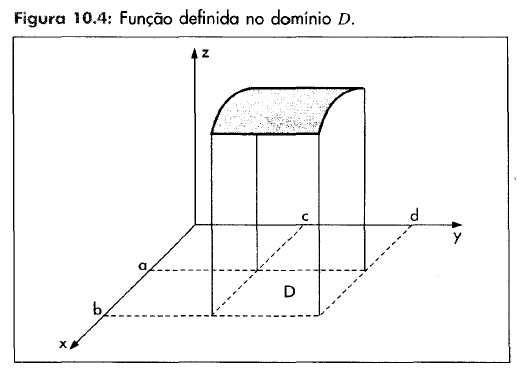
\includegraphics[height=7.5cm]{images/morettin_figura-10-4}
			\end{figure}

			Ao calcularmos a integral parcial (em relação a $y$) $A(x)$, entre $c$ e $d$, estaremos mantendo $x$ constante. Assim, $A(x)$ representará a área da secção do gráfico da função, perpendicular ao eixo $x$, num ponto genérico entre $a$ e $b$. Isto é, $A(x) = \int \limits^{d}_{c} f(x, y)dy$ (Figura 10.5).

			\begin{figure}[H]
				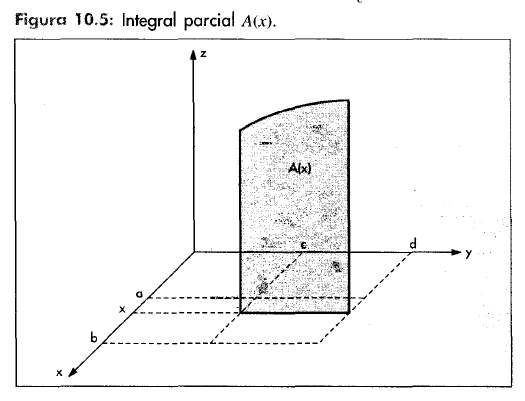
\includegraphics[height=7.5cm]{images/morettin_figura-10-5}
			\end{figure}

			O produto $A(x)dx$ representa o volume do sólido de área $A(x)$ e espessura $dx$. Assim, a integral de $A(x)$ em relação a $x$ representará o volume do sólido sob o gráfico de $f(x, y)$, acima do domínio $D$.

			A esse volume damos o nome de integral dupla de $f(x, y)$ no domínio $D$. Dessa forma, indicando por $V$ o volume do referido sólido, teremos

			\medskip

			$V = \int \limits^{b}_{a} A(x)dx$ .

			\medskip

			Simbolizando a integral dupla por $\int \int_{D} f(x, y)dxdy$, podemos escrever:

			\bigskip

			{\LARGE $\iint_{D} f(x, y)dxdy = \int \limits^{b}_{a} \left[ \int \limits^{d}_{c} f(x, y)dy \right] dx$} . 

			\bigskip

			Poderíamos também ter calculado a área de uma secção perpendicular ao eixo $y$, $B(y)$, da seguinte forma

			\medskip

			$B(y) = \int \limits^{b}_{a} f(x, y)dx$ ,

			\medskip

			e em seguida calculado o volume do sólido sob o gráfico da função e acima do domínio $D$ por

			\medskip

			$V = \int \limits^{d}_{c} B(y)dy = \int \limits^{d}_{c} \left[ \int \limits^{b}_{a} f(x, y)dx \right] dy$ .

			\bigskip

			\textbf{Exemplo}. Consideremos a função $f(x, y) = x + y$, definida no domínio $D$ dado pelas inequações $0 \leq x \leq 5$ e $0 \leq y \leq 3$ e calculemos a integral dupla $\iint _{D} f(x, y)dxdy$, ou seja, o volume $V$ do sólido sob o gráfico da função e acima de $D$.

			\medskip

			a) Primeiro modo

			\medskip

			$A(x) = \int \limits^{3}_{0} (x + y)dy = \left[ xy + \cfrac{y^{2}}{2} \right]^{3}_{0} = 3x + \cfrac{9}{2}$ ,

			$V = \int \limits^{5}_{0} \left( 3x + \cfrac{9}{2} \right) dx = \left[ \cfrac{3x^{2}}{2} + \cfrac{9}{2} x \right]^{5}_{0} = \cfrac{75}{2} + \cfrac{45}{2} = 60$ .

			\bigskip

			b) Segundo modo

			\medskip

			$B(y) = \int \limits^{5}_{0} (x + y)dx = \left[ \cfrac{x^{2}}{2} + xy \right]^{5}_{0} = \cfrac{25}{2} + 5y$ ,

			$V = \int \limits^{3}_{0} \left( \cfrac{25}{2} + 5y \right) dy = \left[ \cfrac{25y}{2} + \cfrac{5y^{2}}{2} \right]^{3}_{0} = \cfrac{75}{2} + \cfrac{45}{2} = 60$.

			\bigskip

			Uma outra situação que ocorre no cálculo da integral dupla é aquela em que o domínio $D$ da função é dado por

			\medskip

			$a \leq x \leq b$

			\smallskip

			e

			\smallskip

			$y_{1}(x) \leq y \leq y_{2}(x)$

			\medskip

			Veja a Figura 10.6.

			\begin{figure}[H]
				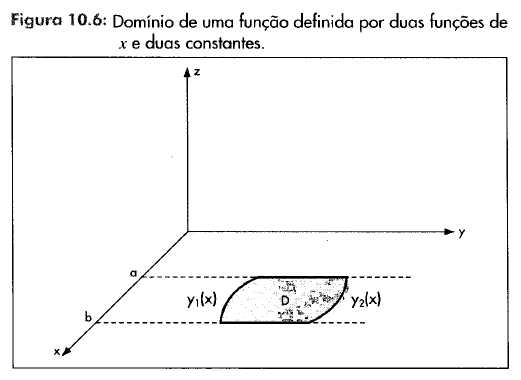
\includegraphics[height=7cm]{images/morettin_figura-10-6}
			\end{figure}

			O $1^{o}$ passo para o cálculo da integral dupla consiste em acha a área $A(x)$ de uma secção do gráfico perpendicular ao eixo $x$, $A(x) = \int \limits^{y_{2}(x)}_{y_{1}(x)} f(x, y)dy$ (Figura 10.7).

			\begin{figure}[H]
				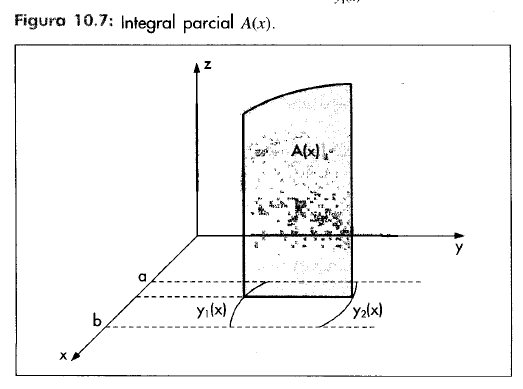
\includegraphics[height=7cm]{images/morettin_figura-10-7}
			\end{figure}

			No $2^{o}$ passo, o volume sob o gráfico e acima do domínio $D$, é dado por

			\medskip

			$V = \int \limits^{b}_{a} A(x)dx$ .

			\medskip

			Portanto, a integral dupla de $f(x, y)$ em $D$ é dada por

			\medskip

			$\iint_{D} f(x, y)dxdy = \int \limits^{b}_{a} \left[ \int \limits^{y_{2}(x)}_{y_{1}(x)} f(x, y)dy \right] dx$ .

			\bigskip

			\textbf{Exemplo}. Seja $f(x, y) = 1$ e $D$  a região dada pelas inequações $0 \leq x \leq 1$ e $x^{2} \leq y \leq x$. Calculemos o volume sólido sob o gráfico da função acima de $D$.

			A região $D$ é dada pela Figura 10.8.

			\begin{figure}[H]
				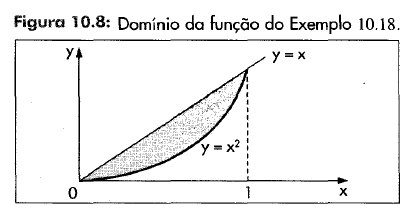
\includegraphics[height=5cm]{images/morettin_figura-10-8}
			\end{figure}

			Temos

			\medskip

			$A(x) = \int \limits^{x}_{x^{2}} 1dy = [y]^{x}_{x^{2}} = x - x^{2}$ ,

			$V = \int \limits^{1}_{0} (x - x^{2})dx = \left[ \cfrac{x^{2}}{2} - \cfrac{x^{3}}{3} \right]^{1}_{0} = \cfrac{1}{2} - \cfrac{1}{3} = \cfrac{1}{6}$ .

			\bigskip

			Uma terceira situação que ocorre no cálculo da integral dupla é aquela em que o domínio $D$ de $f(x, y)$ é dado por

			\medskip

			$c \leq y \leq d$

			\smallskip

			e

			\smallskip

			$x_{1}(y) \leq x \leq x_{2}(y)$

			\medskip

			Veja a Figura 10.9

			\begin{figure}[H]
				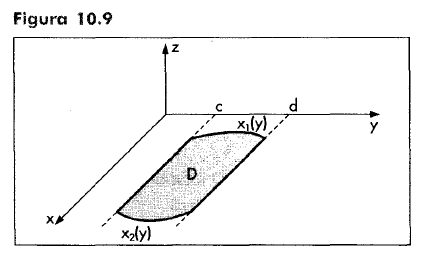
\includegraphics[height=5.5cm]{images/morettin_figura-10-9}
			\end{figure}

			O $1^{o}$ passo para calcular a integral dupla consiste em achar a área $B(y)$ de uma secção do gráfico da função perpendicular ao eixo $y$. Isto é

			\medskip

			$B(y) = \int \limits^{x_{2}(y)}_{x_{1}(y)} f(x, y)dx$ (Figura 10.10).

			\begin{figure}[H]
				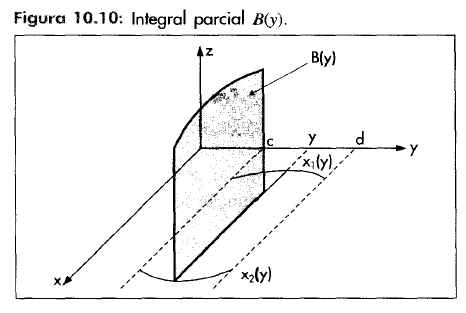
\includegraphics[height=7cm]{images/morettin_figura-10-10}
			\end{figure}

			O $2^{o}$ passo consiste em calcular o volume sob o gráfico de $f(x, y)$ e acima $D$, por meio da integral

			\medskip

			$V = \int \limits^{d}_{c} f(x, y)dy$ .

			\medskip

			Portanto, a integral dupla de $f(x, y)$ em $D$ é dada por

			\medskip

			$\iint_{D} f(x, y)dxdy = \int \limits^{d}_{c} \left[ \int \limits^{x_{2}(y)}_{x_{1}(y)} f(x, y)dx \right] dy$ .

			\bigskip

			\textbf{Exemplo}. Consideremos a função $f(x, y) = x + y$ e calculemos a integral dupla $\iint_{D} f(x, y)dxdy$, em que a região $D$ é dada por

			\medskip

			$1 \leq y \leq 2$

			\smallskip

			e

			\smallskip

			$y \leq x \leq 3y$ .

			\medskip

			Temos

			\medskip

			$B(y) = \int \limits^{3y}_{y} (x + y)dx = \left[ \cfrac{x^{2}}{2} + xy \right]^{3y}_{y} = \cfrac{9y^{2}}{2} + 3y^{2} - \cfrac{y^{2}}{2} - y^{2} = 6y^{2}$ ,

			$V = \int \limits^{2}_{1} 6y^{2}dy = [2y^{3}]^{2}-{1} = 2 \times (8) - 2 \times (1) = 14$ .

			\medskip

			Portanto, a integral dupla procurada vale 14.

			\bigskip

			\textbf{Observações}

			\begin{enumerate}[label=\alph*)]

				\item De modo geral, se o domínio $D$ não puder ser expresso de acordo com as situações descritas, então subdividimos o domínio em partes tais que cada uma se enquadre nos casos dados.

				\item Nos casos estudados, consideramos $f(x, y) \geq 0$; caso tenhamos $f(x, y) \leq 0$, então $-f(x, y) \geq 0$. Assim, a integral dupla da função será o oposto do volume do sólido compreendido entre $D$ e o gráfico da função.
				
			\end{enumerate}

		\section{Máximos e Mínimos para Funções de Duas Variáveis}

		\subsection{Definições \cite{morettin}}

		Uma importante aplicação do estudo das derivadas parciais é a otimização de funções. Otimizar uma função significa encontrar seu ponto de máximo ou de mínimo. Assim, determinar a máxima produção de um firma com um dado orçamento constitui um problema de maximização; entre possíveis combinações de insumos, aquela que nos permite obter certo nível de produção, a custo mínimo, consiste em resolver um problema de minimização. Vamos tornar mais precisas essas ideias, com algumas definições.

		Seja $f$ uma função de duas variáveis $x$ e $y$. Dizemos que um ponto $(x_{0}, y_{0})$ do domínio $D$ é um ponto de máximo relativo de $f$, ou simplesmente \textbf{ponto de máximo}, se existir uma bola aberta de centro $(x_{0}, y_{0})$ e raio $r$, tal que, para todo ponto $P(x, y)$ do domínio situado no interior dessa bola aberta, tenhamos

		\medskip

		$f(x, y) \leq f(x_{0}, y_{0})$

		\medskip

		[Lembre-se que $f(x, y) = z$, logo estamos trabalhando com uma bola aberta de centro $(x_{0}, y_{0})$ e raio $r$ no plano $xOy$].

		\medskip

		Ao número $f(x_{0}, y_{0})$ damos o nome de valor máximo de $f$ (Figura 11.1).

		\begin{figure}[H]
				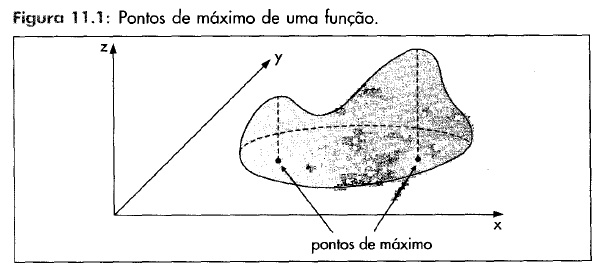
\includegraphics[height=6.5cm]{images/morettin_figura-11-1}
		\end{figure}

		Analogamente, dizemos que um ponto $(x_{0}, y_{0})$ do domínio $D$ é um ponto de mínimo relativo de $f$, ou simplesmente \textbf{ponto de mínimo}, se existir uma bola aberta de centro $(x_{0}, y_{0})$ e raio $r$, tal que, para todo ponto $P(x, y)$ do domínio situado no interior dessa bola aberta de centro $(x_{0}, y_{0})$ e raio $r$, tal que, para todo ponto $P(x, y)$ do domínio situado no interior dessa bola aberta, tenhamos

		\medskip

		$f(x, y) \geq f(x_{0}, y_{0})$ .

		\medskip

		Ao número $f(x_{0}, y_{0})$ damos o nome de valor mínimo de $f$ (Figura 11.2).

		\begin{figure}[H]
				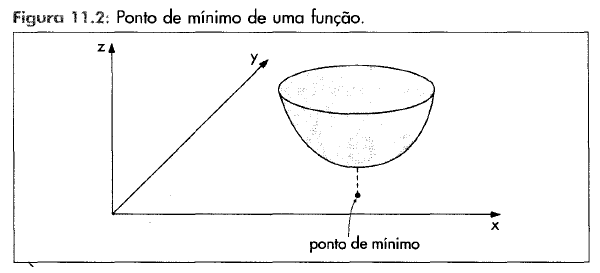
\includegraphics[height=6.5cm]{images/morettin_figura-11-2}
		\end{figure}

		Seja $f$ um função de duas variáveis $x$ e $y$. Dizemos que um ponto $(x_{0}, y_{0})$ do domínio $D$ é um ponto de \textbf{máximo global (ou absoluto)} de $f$ se, para todo ponto $P(x, y)$ do domínio tivermos

		\medskip

		$f(x, y) \leq f(x_{0}, y_{0})$ .

		\medskip

		Analogamente, dizemos que um ponto $(x_{0}, y_{0})$ do domínio $D$ é um ponto de \textbf{mínimo global (ou absoluto)} de $f$ se, para todo ponto $P(x, y)$ do domínio, tivermos

		\medskip

		$f(x, y) \geq f(x_{0}, y_{0})$ .

		\medskip

		A descoberta de um ponto de máximo ou de mínimo exige, na maioria dos casos, o conhecimento do gráfico de $f$, o que, conforme vimos, não é um problema fácil.

		Entretanto, existem teoremas que nos auxiliam nesse sentido, e que passaremos a estudar.

		\bigskip

		\textbf{Teorema 11.1} \cite{morettin}

		\medskip

		Seja $f$ uma função com duas variáveis $x$ e $y$ e seja $(x_{0}, y_{0})$ um ponto interior ao domínio.
		Se $(x_{0}, y_{0})$ for um ponto de máximo ou de mínimo de $f$ e se existirem derivadas parciais $fx$ e $fy$, então

		\medskip

		$fx(x_{0}, y_{0}) = 0$ \ e \ $fy(x_{0}, y_{0}) = 0$ .

		\bigskip

		\textbf{Demonstração}

		\medskip

		Suponhamos que $(x_{0}, y_{0})$ seja um ponto de máximo. Existe a bola aberta de centro $(x_{0}, y_{0})$ e raio $r$, no interior do domínio $D$, cujos pontos $(x, y)$ são tais que $f(x, y) \leq f(x_{0}, y_{0})$ (Figura 11.3).

		\begin{figure}[H]
				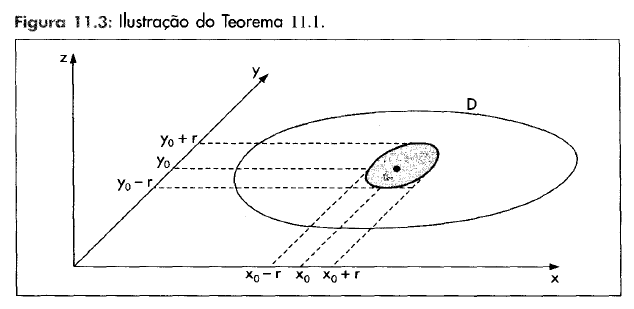
\includegraphics[height=6.5cm]{images/morettin_figura-11-3}
		\end{figure}

		Consideremos os pontos dessa bola para os quais $y = y_{0}$. Então $f(x, y_{0})$ será função somente de $x$. Mas, como $f(x, y_{0}) \leq f(x_{0}, y_{0})$ para $x_{0} - r < x < x_{0} + r$, segue-se que a função $f(x, y_{0})$ de uma variável tem um ponto de máximo em $(x_{0}, y_{0})$ e, consequentemente, $fx(x_{0}, y_{0}) = 0$.

		Analogamente, se considerarmos os pontos da bola aberta para os quais $x = x_{0}$, então $f(x_{0}, y)$ será só função de $y$. Mas, como $f(x_{0}, y) \leq f(x_{0}, y_{0})$ para $y_{0} - r < y < y_{0} + r$, segue-se que a função $f(x_{0}, y)$, de uma variável, tem um ponto máximo em $(x_{0}, y_{0})$ e, consequentemente $fy(x_{0}, y_{0}) = 0$.

		Em resumo, \textbf{se $\boldsymbol{(x_{0}, y_{0})}$ for ponto de máximo, então $\boldsymbol{fx(x_{0}, y_{0}) = 0}$ \ e \ $\boldsymbol{fy(x_{0}, y_{0}) = 0}$}.

		Os pontos que anulam simultaneamente as derivadas parciais $fx$ e $fy$ são chamados \textbf{pontos críticos de $f$}.

		\bigskip

		\textbf{Observações}

		\medskip

		Antes de prosseguirmos, cumpre salientarmos algumas considerações bastante importantes em tudo que segue.

		\begin{enumerate}[label=(\roman*)]

			\item O Teorema não nos garante a existência de pontos de máximo ou de mínimo, mas sim \textbf{possíveis [candidatos] pontos de máximo ou mínimo}. Assim, pode ocorrer de termos $fx(x_{0}, y_{0}) = 0$ \ e \ $fy(x_{0}, y_{0}) = 0$ sem que $(x_{0}, y_{0})$ seja ponto de máximo ou mínimo.

			Um exemplo desse fato é o da função $f(x, y) = xy$, em que $fx = y$ e $fy = x$; o ponto crítico é $(0, 0)$.

			Assim, se tomarmos uma bola aberta de centro $(0, 0)$ e raio $r$, teremos:

			\begin{enumerate}[label=\alph*)]

				\item para os pontos dessa bola aberta situados no interior do primeiro e terceiro quadrantes, $f(x, y) = xy > 0$, pois $x$ e $y$ têm o mesmo sinal;

				\item para os pontos dessa bola aberta situados no interior do segundo e quarto quadrantes $f(x, y) = xy < 0$, pois $x$ e $y$ têm sinais contrários.

			\end{enumerate}

			Logo

			\medskip

			$(0,0)$ não é ponto de máximo nem de mínimo.

			\medskip

			Verifica-se que o gráfico dessa função tem o aspecto de uma $sela de cavalo$. O ponto $(0, 0)$ é chamado de \textbf{ponto de sela} (Figura 11.4).

			\begin{figure}[H]
				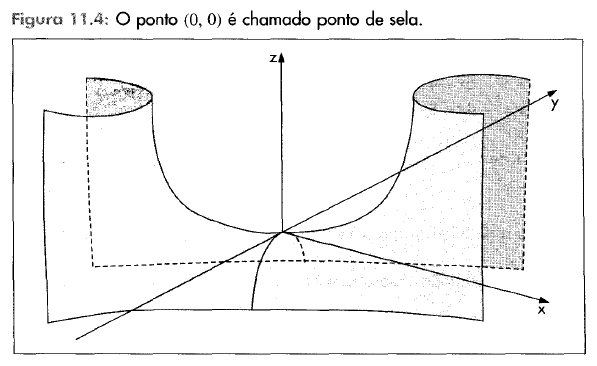
\includegraphics[height=7cm]{images/morettin_figura-11-4}
			\end{figure}

			\begin{figure}[H]
				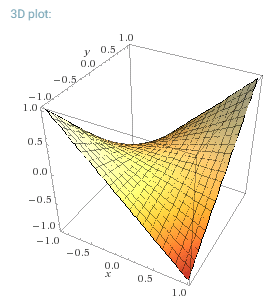
\includegraphics[height=7cm]{images/wolframalpha_figura-1-1}
				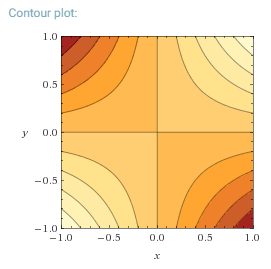
\includegraphics[height=7cm]{images/wolframalpha_figura-1-2} \cite{wolframalpha}
			\end{figure}

			De um modo geral, todo ponto crítico $(x_{0}, y_{0})$ que não é de máximo nem de mínimo é chamado ponto de sela.

			Encontramos um problema semelhante com qualquer plano horizontal em $xOz$. Planos horizontais não têm um único ponto de máximo ou de mínimo, pois qualquer ponto pode ser considerado máximo e mínimo ao mesmo tempo $f(x, y) = f (x_{0}, y_{0})$.

			\item O Teorema só se aplica a pontos interiores do domínio. Assim, os pontos que anulam as derivadas parciais $fx$ e $fy$ só podem ser pontos de máximo ou mínimo do interior do domínio. A análise dos pontos de fronteira deve ser feita à parte, como veremos a seguir.

		\end{enumerate}

	\subsection{Critérios para Identificação de Pontos de Máximo ou Mínimo \cite{morettin}}

		O Teorema 11.1 permitiu-nos determinar os possíveis pontos de máximo ou de mínimo no interior do domínio, sem, contudo, identificá-los. O Teorema 11.2, que veremos a seguir, permitirá esta identificação. Sua demonstração poderá ser vista, por exemplo, em Leithold (1977).

		\bigskip

		\textbf{Teorema 11.2} \cite{morettin}

		\medskip

		Seja $f$ uma função de duas variáveis $x$ e $y$, contínua, com derivadas parciais até segunda ordem contínuas. Seja $(x_{0}, y_{0})$ um ponto crítico de $f$. Chamemos o determinante

		\medskip

		$
		H(x_{0}, y_{0}) =
		\begin{vmatrix}

			fxx(x_{0}, y_{0}) & fxy(x_{0}, y_{0}) \\
			fyx(x_{0}, y_{0}) & fyy(x_{0}, y_{0})

		\end{vmatrix}
		$

		\medskip

		de Hessiano ($H$) (em homenagem ao matemático alemão Ludwig Otto Hesse, 1811-1874) de $f$ no ponto $(x_{0}, y_{0})$. Se:

		\begin{enumerate}[label=(\alph*)]

			\item $H(x_{0}, y_{0}) > 0$ e $fxx(x_{0}, y_{0}) < 0$, então $(x_{0}, y_{0})$ será ponto de máximo de $f$,

			\item $H(x_{0}, y_{0}) > 0$ e $fxx(x_{0}, y_{0}) > 0$, então $(x_{0}, y_{0})$ será ponto de mínimo de $f$,

			\item $H(x_{0}, y_{0}) > 0$, então $(x_{0}, y_{0})$ será ponto de sela de $f$.

		\end{enumerate}
		
	\subsection{Uma Aplicação: Ajuste de Retas pelo Método dos Mínimos Quadrados \cite{morettin}}
	
	\subsection{Análise dos Pontos de Fronteira \cite{morettin}}

		Até agora, vimos como encontrar máximos e mínimos de funções analisando apenas os pontos interiores ao domínio (pois os teoremas dados só se aplicam a esses pontos). A análise dos pontos de fronteira (quando existem) terá que ser feita sem o auxílio destes teoremas. Uma das formas usadas para abordar tais situações é por meio das curvas de nível da função a ser otimizada. Os exemplos esclarecerão este tipo de abordagem.

		\bigskip

		\textbf{Exemplo}. Consideremos a função $f$ dada por $f(x, y) = 2x + y$, definida no domínio $D$ dado pelas inequações

		\medskip

		$x \geq 0$, \\
		$y \geq 0$, \\
		$x + y \leq 7$.

		\begin{enumerate}[label=\alph*)]

			\item Em primeiro lugar, notemos que o conjunto $D$ é constituído pela reunião do triângulo da Figura 11.9 com sua parte interna. A fronteira do domínio é constituída dos lados $\overline{AB}$, $\overline{BC}$ e $\overline{AC}$.

			\begin{figure}[H]
				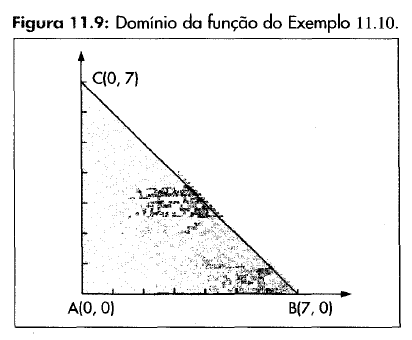
\includegraphics[height=7cm]{images/morettin_figura-11-9}
			\end{figure}

			\item A função $f(x, y) = 2x + y$ admite como curvas de nível o feixe de paralelas à reta $2x + y = 0$, pois qualquer curva de nível $c$ tem por equação a reta $2x + y = c$, que é paralela à $2x + y = 0$ qualquer que seja $c$.

			Eis algumas curvas de nível. Seus gráficos comparecem na Figura 11.10:

			\medskip

			$c = 1 \rightarrow 2x + y = 1$ \\
			$c = 2 \rightarrow 2x + y = 2$ \\
			$c = 3 \rightarrow 2x + y = 3$ .

			\begin{figure}[H]
				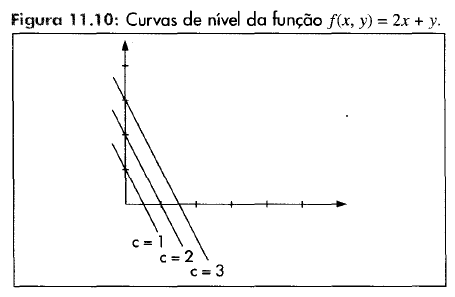
\includegraphics[height=6cm]{images/morettin_figura-11-10}
			\end{figure}

			\begin{figure}[H]
				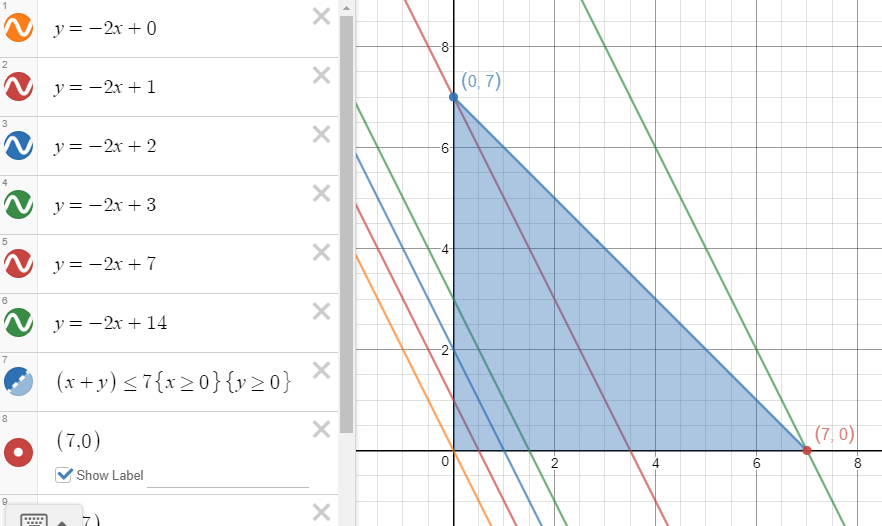
\includegraphics[height=7cm]{images/desmos_figura-1} \cite{desmos}
			\end{figure}

			Notemos, nesse exemplo, que, quanto mais a reta se distancia da origem, maior é o valor de $c$.

			\item Como todos os pontos $(x, y)$ da curva de nível $c$ produzem um valor constante para $f(x, y)$, o ponto da curva de maior nível que intercepta $D$ é o ponto de máximo de $f$; no caso do exemplo em questão, tal ponto é $B(7, 0)$. A curva de menor nível que intercepta $D$ é o ponto de mínimo de $f$; no caso, tal ponto é $A(0, 0)$ (Figura 11.11).

			\begin{figure}[H]
				\includegraphics[height=8cm]{images/morettin_figura-11-11}
			\end{figure}

			\item O ponto $(0, 0)$ é o ponto de mínimo absoluto e $(7, 0)$ é o ponto de máximo absoluto de $f$.

			\item Entre os pontos interiores a $D$, não existem pontos de máximo ou mínimo, pois as derivadas parciais nunca se anulam ($fx = 2$ e $fy = 1$).

		\end{enumerate}

		É intuitivo perceber, nesse exemplo, que os pontos de máximo ou mínimo estão nos vértices do triângulo. Assim, por simples inspeção do valor de $f$ nos pontos $A$, $B$ e $C$, poderíamos descobrir os pontos de máximo e mínimo.
			De fato,

		\medskip

		$f(x, y) = 2x + y$, \\
		$A(0, 0) \rightarrow f(0, 0) = 2 \times 0 + 0 = 0$, \\
		$B(7, 0) \rightarrow f(7, 0) = 2 \times 7 + 0 = 14$, \\
		$C(0, 7) \rightarrow f(0, 7) = 2 \times 0 + 7 = 7$,

		\medskip

		e, portanto, $A(0, 0)$ é o ponto de mínimo e $B(7, 0)$ é o ponto de máximo de $f$.

		\bigskip

		\textbf{Exemplo}. Consideremos a função dada por $f(x, y) = x + y$, definida no domínio $D$ determinado pelas inequações

		\medskip

		$x \geq 0$, \\
		$y \geq 0$, \\
		$2x + y \geq 10$, \\
		$x + 2y \geq 10$.

		\medskip

		\begin{enumerate}[label=\alph*)]

			\item O conjunto $D$ é formado pelos pontos da região indicada na Figura 11.12.

			\begin{figure}[H]
				\includegraphics[height=7cm]{images/morettin_figura-11-12}
			\end{figure}

			Os pontos $A$, $B$ e $C$ têm coordenadas $(0, 10)$, $\left( \cfrac{10}{3}, \cfrac{10}{3} \right)$ e $(10, 0)$ respectivamente; o ponto $B$ é a intersecção das retas $2x + y = 10$ e $x + 2y = 10$.

			Os pontos de fronteira do domínio são aqueles dos segmentos $\overline{AB}$ e $\overline{BC}$, bem como os das semi-retas, $\overline{AP}$ e $\overline{CQ}$.

			\item A função $f(x, y) = x + y$ admite como curvas de nível o feixe de retas paralelas à reta $x + y = 0$.

			Eis algumas curvas de nível e seus respectivos gráficos (Figura 11.13):

			\medskip

			$c = 1 \rightarrow x + y = 1$ \\
			$c = 2 \rightarrow x + y = 2$ \\
			$c = 3 \rightarrow x + y = 3$ \\

			\begin{figure}[H]
				\includegraphics[height=7cm]{images/morettin_figura-11-13}
			\end{figure}

			\item O ponto de mínimo de $f$ é o ponto da curva de menor nível que intercepta $D$. Assim, o ponto de mínimo é o ponto $B\left( \cfrac{10}{3}, \cfrac{10}{3} \right)$ (Figura 11.14).

			\begin{figure}[H]
				\includegraphics[height=8cm]{images/morettin_figura-11-14}
			\end{figure}

			\item A função $f$ não tem ponto de máximo em $D$, pois não existe curva de maior nível de $f$ que intercepte $D$ (Figura 11.15).

			\begin{figure}[H]
				\includegraphics[height=9cm]{images/morettin_figura-11-15}
			\end{figure}

		\end{enumerate}

		\textbf{Exemplo}. Consideremos a função dada por $f(x, y) = x + y$ e domínio $D$ determinado pelas inequações

		\medskip

		$x \geq 0$, \\
		$y \geq 0$, \\
		$x + y \leq 3$.

		\medskip

		\begin{enumerate}[label=\alph*)]

			\item O conjunto $D$ é constituído pela região triangular da Figura 11.16. Os vértices do triângulo são $A(0, 0)$, $B(3, 0)$ e $C(0, 3)$.

			\begin{figure}[H]
				\includegraphics[height=6cm]{images/morettin_figura-11-16}
			\end{figure}

			\item A função dada admite como curvas de nível o feixe de paralelas à reta $x + y = 0$ (Figura 11.17).

			\item Todos os pontos do segmento $\overline{BC}$ são pontos de máximo, pois a reta determinada por $\overline{BC}$ tem o mesmo coeficiente angular que o feixe de paralelas $(-1)$. O ponto de mínimo de $f$ é o ponto $A(0, 0)$ (Figura 11.18).

			\begin{figure}[H]
				\includegraphics[height=7cm]{images/morettin_figura-11-17}
				\includegraphics[height=7cm]{images/morettin_figura-11-18}
			\end{figure}

		\end{enumerate}

		\textbf{Exemplo}. Determine o ponto de máximo e mínimo da função $f(x, y) = x + y$ no domínio dado por $D = \{(x, y) \in \mathbb{R} \mid x^{2} + y^{2} \leq 1\}$.

		\medskip

		O domínio da função é o círculo de centro na origem e raio $1$ (Figura 11.19).

		As curvas de nível da função são as retas do feixe de paralelas $x + y = c$ (Figura 11.20).

		Portanto, os pontos de máximo e de mínimo são os pontos de tangência de $x + y = c$ com a circunferência $x^{2} + y^{2} = 1$ (Figura 11.21).

		\begin{figure}[H]
			\includegraphics[height=5cm]{images/morettin_figura-11-19}
			\includegraphics[height=5cm]{images/morettin_figura-11-20}
			\includegraphics[height=5cm]{images/morettin_figura-11-21}
		\end{figure}

		Assim sendo, devemos impor que o sistemas de equações

		\bigskip

		$
		\begin{cases}
			x + y = c & (11.1)\\
			x^{2} + y^{2} = 1 & (11.2)
		\end{cases}
		$

		\bigskip

		tenha solução única.

		\medskip

		De (11.1) temos $y = c - x$. Substituindo em (11.2), teremos:

		\medskip

		$2x^{2} - 2cx + c^{2} - 1 = 0$ \ \ (11.3)

		\medskip

		Para que (11.3) tenha uma única raiz, seu discriminante ($\Delta$) deve ser nula. Assim:

		\medskip

		$\Delta = 4c^{2} - 8(c^{2} -1) = -4c^{2} + 8 = 0 \implies c = \sqrt{2} \ \text{ou} \ c = - \sqrt{2}$

		\medskip

		É evidente que para $c = \sqrt{2}$ teremos um ponto de máximo e para $c = - \sqrt{2}$ teremos um ponto de mínimo.

		Para $c = \sqrt{2}$ a equação (11.3) fica igual a $2x^{2} - 2\sqrt{2}x + 1 = 0$, cuja raiz é $x = \cfrac{\sqrt{2}}{2}$.

		O valor de $y$ é dado pela equação (11.1), isto é: $y = \sqrt{2} - \cfrac{\sqrt{2}}{2} = \cfrac{\sqrt{2}}{2}$. Portanto o ponto de máximo é $\left( \cfrac{\sqrt{2}}{2}, \cfrac{\sqrt{2}}{2} \right)$.

		Para $c = - \sqrt{2}$ concluímos de modo análogo que o ponto de mínimo é $\left( - \cfrac{\sqrt{2}}{2}, - \cfrac{\sqrt{2}}{2} \right)$.
		
	\subsection{Máximos e Mínimos Condicionados \cite{morettin}}
	
		\subsubsection{Método da Substituição \cite{morettin}}

		\subsubsection{Método dos Multiplicadores de Lagrange \cite{morettin}}

		\section{Funções de Três ou Mais Variáveis}

		\section{Matrizes e Determinantes}

		\section{Sistemas de Equações}

	\pagebreak

\begin{thebibliography}{}

\bibitem{desmos}
DESMOS.
Disponível em: $<$https://www.desmos.com/$>$.

\bibitem{google}
GOOGLE IMAGENS.
Disponível em: $<$https://images.google.com.br/$>$.

\bibitem{lucchesi}
LUCCHESI, Andrea

\bibitem{morettin}
MORETTIN, Pedro A; HAZZAN, Samuel; BUSSAB, Wilton de O.
Cálculo - funções de uma e várias variáveis.
1 ed.
São Paulo:
Saraiva, \
2003.

\bibitem{somatematica}
SÓ MATEMÁTICA.
Disponível em: $<$http://www.somatematica.com.br/$>$.

\bibitem{symbolab}
SYMBOLAB.
Disponível em: $<$https://www.symbolab.com/$>$.

\bibitem{ufmg}
UNIVERSIDADE FEDERAL DE MINAS GERAIS.
Disponível em: $<$http://www.mat.ufmg.br/$>$.

\bibitem{ventura}
VENTURA, Marcelo F.

\bibitem{wikipedia}
WIKIPEDIA.
Disponível em: $<$https://www.wikipedia.org/$>$.

\bibitem{wolframalpha}
WOLFRAMALPHA.
Disponível em: $<$http://www.wolframalpha.com/$>$.

\end{thebibliography}


\end{document}